\documentclass[runningheads,a4paper,oribibl]{llncs}

\usepackage{amssymb,amsmath}
\setcounter{tocdepth}{3}
\usepackage{graphicx}
\usepackage{url}
\def\UrlBreaks{\do\/\do-}

\newcommand{\keywords}[1]{\par\addvspace\baselineskip
\noindent\keywordname\enspace\ignorespaces#1}

\begin{document}

\mainmatter

\title{A Zone-Aware and Explainable Decision Support Framework\\for Mango Soil--Microbiome Intelligence and\\Yield-Gap Assessment in Uttar Pradesh, India}

\titlerunning{Zone-Aware Explainable Mango Soil--Microbiome DSS}

\author{Research Team\inst{1}}

\authorrunning{Research Team}

\institute{CV Raman Research Work, Uttar Pradesh, India}

\toctitle{Zone-Aware Explainable Mango Soil--Microbiome DSS}
\tocauthor{Research Team}

\maketitle

\begin{abstract}
Mango productivity in Uttar Pradesh is governed by interactions among soil physicochemical factors, rhizosphere microbiome diversity, microclimate, and orchard management. We present a reproducible, zone-aware, explainable decision support framework integrating multi-modal soil-microbiome data to predict mango yield and classify disease risk and soil nutrient availability. The empirical dataset comprises $20{,}000$ samples across $63$ attributes from $50$ commercial orchards in four Lucknow blocks (Malihabad, Kakori, Mall, Rahimabad). Model evaluation employs internal 5-fold cross-validation, orchard-aware GroupKFold, and spatial geographic hold-out evaluation using Rahimabad ($5{,}059$ samples). Selected champions include Linear Regression for yield (geographic RMSE 1.984 kg/tree; MAE 1.594; $R^2 \approx 0.273$), Gradient Boosting for disease risk (macro-F1 $0.990$), and Random Forest for nutrient availability (macro-F1 $0.9998$). Explainable AI attributions via SHAP and LIME, combined with local $Q_{75}$ attainable benchmarks, provide transparent agronomic diagnostics delivered through bilingual API and dashboard interfaces.

\keywords{Mango, soil microbiome, decision support system, explainable AI, SHAP, LIME, geographic hold-out, orchard-grouped validation, yield gap, Uttar Pradesh}
\end{abstract}


\section{Introduction}

\subsection{Agricultural and Scientific Context}
Beyond this, mango (\textit{Mangifera indica L.}) is any second premier horticultural crop in India\cite{berendsen2012,mendes2011}, holding huge economic and nutritional significance, especially within the alluvial Gangetic plains of Uttar Pradesh, to a significant degree; in fact, the Malihabad region is known globally for its premium mango cultivars, such as Dashehari, Chausa, Langra and Lucknow Safeda, in actual application. Nonetheless, orchard productivity is revealing major spatial and temporal variability owing to mixed soil fertility, salinity, sub-soil moisture dynamics, microclimatic fluctuations\cite{bouskill2013}, tree age structures, and rhizosphere microbiome diversity\cite{singh2020}.

Soil health and rhizosphere microbial communities play the foundational part in nutrient cycling, pathogen suppression, and plant vigor, on the whole. In light of this dynamic, good guilds spanning nitrogen-fixing bacteria, phosphate-solubilizing bacteria (PSB), arbuscular mycorrhizal fungi (AMF), and plant-growth-promoting rhizobacteria (PGPR) interact synergistically with soil physicochemical characteristics (pH, organic carbon, available NPK, micronutrients) to evaluate tree productivity and toughness against fungal pathogens such as \textit{Fusarium} wilt and anthracnose, in real-world scenarios. Despite their critical importance, high-dimensional soil-microbiome data are complex and challenging\cite{fierer2017,bahram2018} for growers to construe intuitively, creating one urgent need for an integrated, quantitative and explainable decision support system (DSS).

\subsection{Decision-Support Problem}
A solid DSS must fulfill six core capabilities: (1) exactly estimate possible tree yield, under the local soil-climatic conditions; (2) classify orchard disease risk and nutrient status objectively; (3) transparently explain; (4) benchmark individual orchard performance against local peer cohorts; (5) stringently isolate measured nutrient deficiencies from embodied feature correlations; and (6) prevent inappropriate prescriptive fertilizer dosing formulated directly from black-box feature attributions, broadly speaking. To clarify, effective orchard management is needing moving beyond generalized fertilizer recommendations toward the precision, zone-aware agronomic intelligence, in many respects.

\subsection{Research Gap}
Previous agricultural machine learning studies regularly suffer from several methodological shortcomings - counting exclusively on random row-level train-test splits that are causing spatial information leakage; ignoring orchard-level spatial link directing to pseudo-replication; conflating statistical feature attribution with biological causation; and failing to offer geographic hold-out validation, across the separate agro-ecological sub-zones, in many respects. Against this backdrop, the put forward study tackles all these gaps by starting a leakage-aware modeling pipeline incorporating orchard-grouped validation, spatial geographic hold-out testing, XAI guardrails, and zone benchmark comparisons, to a significant degree.

\subsection{Study Objectives}
\textbf{Primary objective:} To design, implement, and evaluate a reproducible, zone-aware, and explainable decision support framework for mango soil-microbiome intelligence and yield-gap assessment.

\textbf{Secondary objectives:}
(1) Curate and validate a comprehensive $20{,}000$-sample multi-modal dataset spanning soil chemistry, microbiome taxonomy, climate, and orchard metadata.
(2) Develop and optimize multi-task models for yield regression, disease risk classification, and nutrient availability classification.
(3) Evaluate spatial generalization performance using Rahimabad as an independent geographic hold-out zone.
(4) Perform orchard-grouped validation using GroupKFold to account for within-orchard sample correlation.
(5) Generate global and local model explanations using TreeSHAP and LIME with explicit interpretive boundaries.
(6) Translate measured soil-microbiome status into cautious, evidence-tiered agronomic recommendations and bilingual farmer reports.

\subsection{Research Questions}
(1) Can evidently one integrated multi-task modeling pipeline generate solid, reproducible predictions from multi-modal soil-microbiome schemas?
(2) How do model generalization metrics differ between internal cross-validation, orchard-grouped validation, and geographic hold-out check?
(3) Which soil physicochemical and microbial taxa features are, by definition, most influential across the produce, disease and nutrient targets?
(4) Can relatively model explanations be communicated successfully without conflating statistical association with biological causation?
(5) Can generally the zone-aware DSS deliver doable agronomic diagnostics while upholding strict epistemic shortcomings?


\section{Materials and Methods}

\subsection{Study Setting}
The examination concentrates on the major mango-producing agro-ecological blocks of the Lucknow district in Uttar Pradesh, India, such as Malihabad, Rahimabad, Kakori, and Mall, to a significant degree. In light of this dynamic, all the zones represent the core alluvial plain ecosystems characteristic of northern Indian subtropical horticulture, in real-world scenarios.

\begin{figure}[t]
\centering
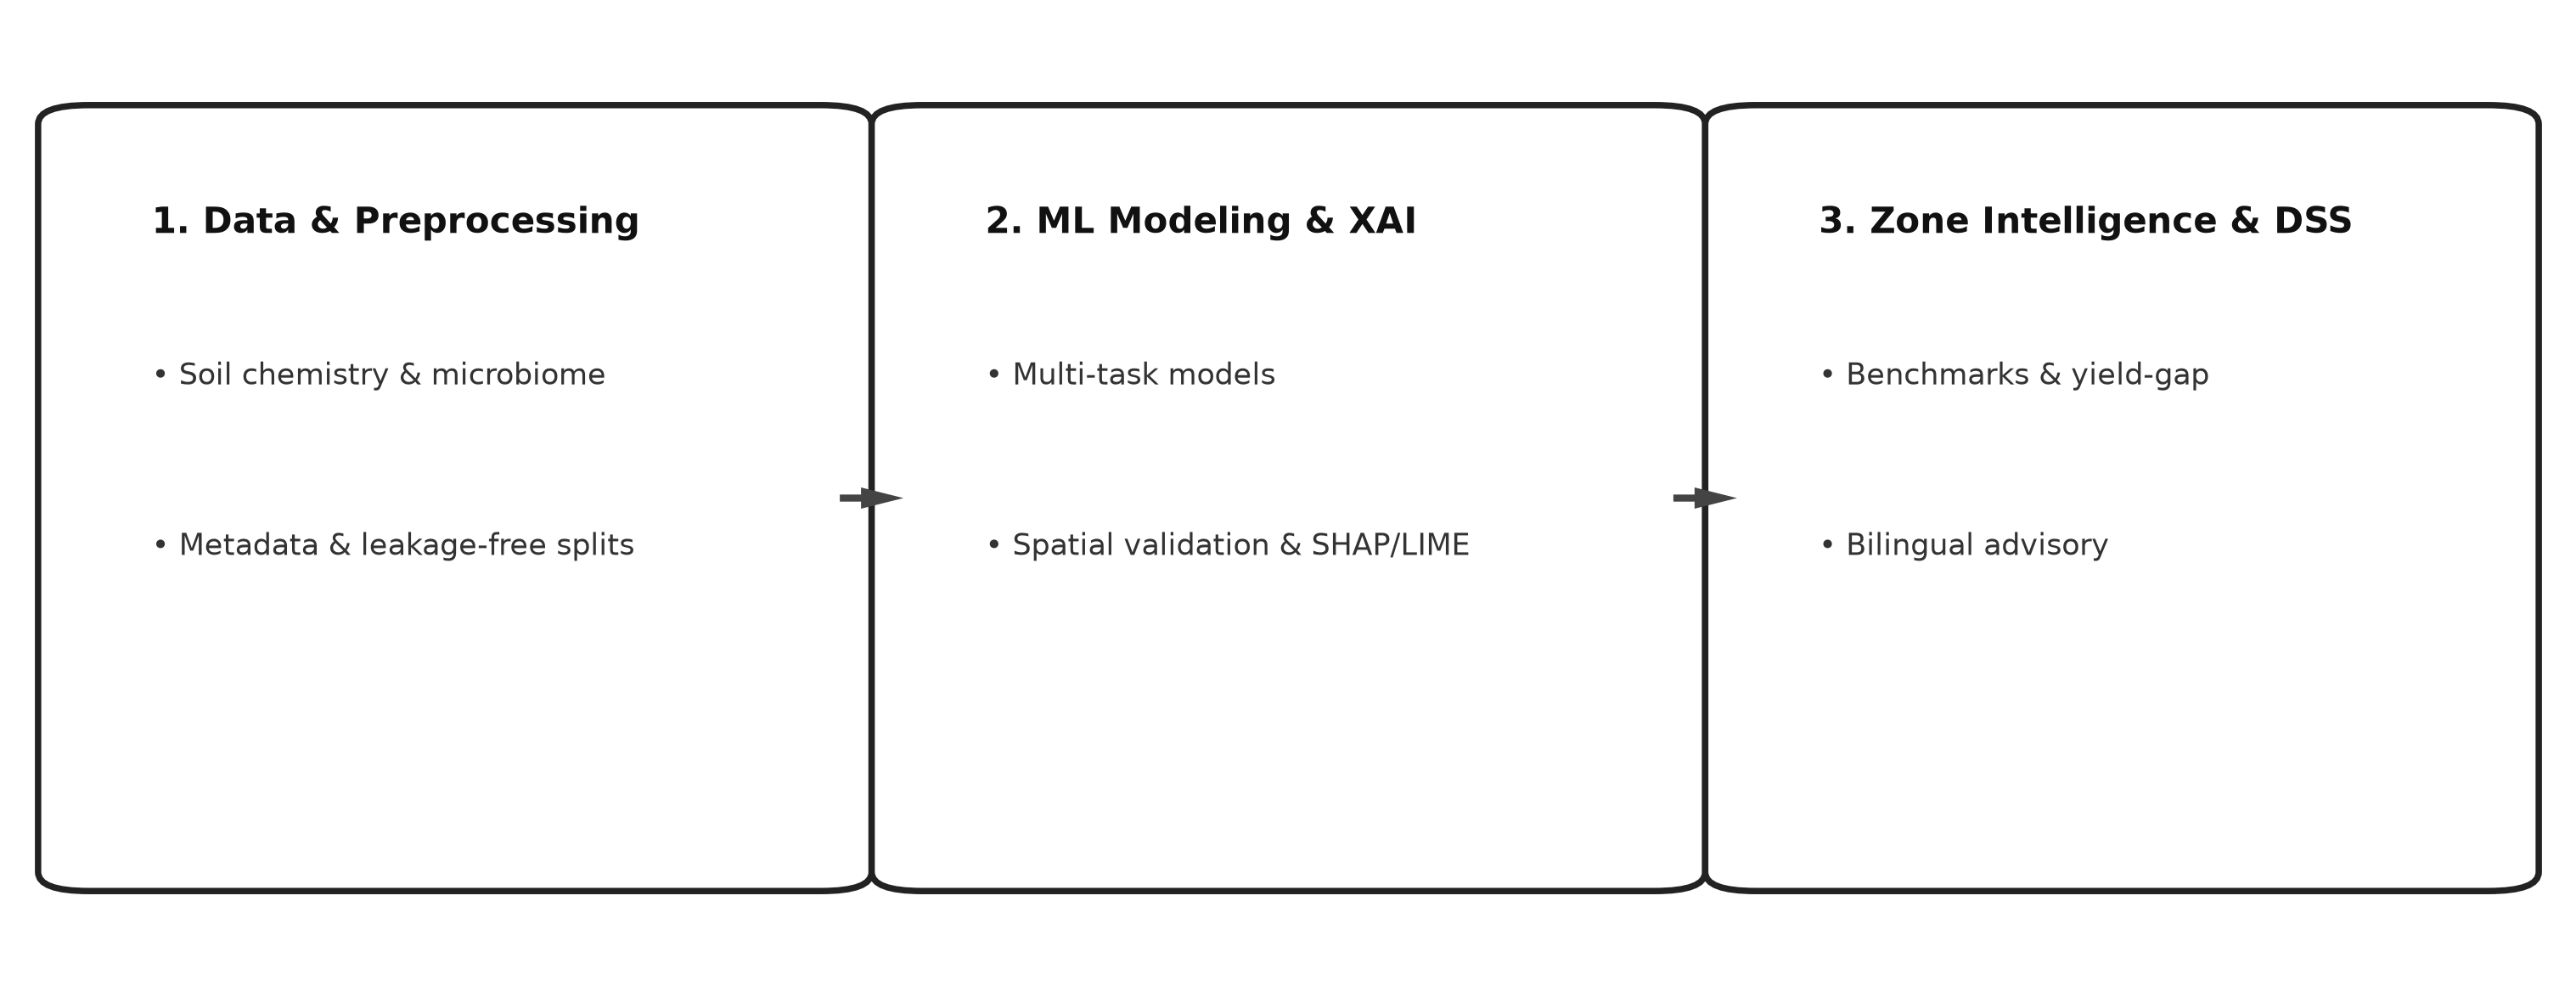
\includegraphics[width=0.92\textwidth]{figures/fig1_framework_architecture.png}
\caption{End-to-end conceptual architecture of the zone-aware, explainable mango decision support framework.}
\label{fig:arch}
\end{figure}

\subsection{Dataset Provenance and Profiling}
The empirical database comprises $20{,}000$ observational samples and $63$ original variables across $50$ commercial orchards ($400$ samples per orchard; $5{,}000$ samples per village). Comprehensive quality audits confirmed zero missing values and zero duplicate records. Following verification, the processed master dataset and modeling feature table containing engineered indicators and split metadata span $20{,}000$ rows $\times$ $84$ columns (stored under \path{data/processed/}). Table~\ref{tab:dataset_schema} summarizes the primary dataset schema.

\begin{table}[t]
\caption{Dataset schema and variable categories.}
\label{tab:dataset_schema}
\centering
\begin{tabular}{lp{6.8cm}c}
\hline
Variable Category & Description & Count \\
\hline
Metadata & Sample ID, Orchard ID, Village, Lat/Long, Variety, Age, Depth, Season, Management & 10 \\
Soil Physicochemical & pH, EC, Organic Carbon, Total N, Avail. P, K, Moisture, Temp, Bulk Density, CEC, Texture, Micronutrients & 18 \\
Climate Metrics & Air Temperature, Rainfall, Humidity, Solar Radiation & 4 \\
Alpha Diversity & OTU Count, Shannon Index, Simpson Index, Chao1 Richness, Pielou Evenness & 5 \\
Microbiome Phyla & Bacterial (5), Fungal (5), Archaeal (2) phyla abundances & 12 \\
Functional Guilds & N-Fixers, PSB, K-Solubilizers, AMF, Trichoderma, Pseudomonas PGPR, Fusarium & 7 \\
Engineered Indices & Pathogen Load Index, Microbial Richness, Nutrient Balance Ratio, Soil Health Index & 14 \\
Targets & Mango Yield (kg/tree), Disease Risk (3 classes), Nutrient Availability (3 classes) & 3 \\
\hline
\end{tabular}
\end{table}

\subsection{Sampling Design and Stratification}
Figure~\ref{fig:spatial} illustrates the spatial and phenological distribution of the study cohort across villages, varieties, tree age cohorts, and sampling depths.

\begin{figure}[t]
\centering
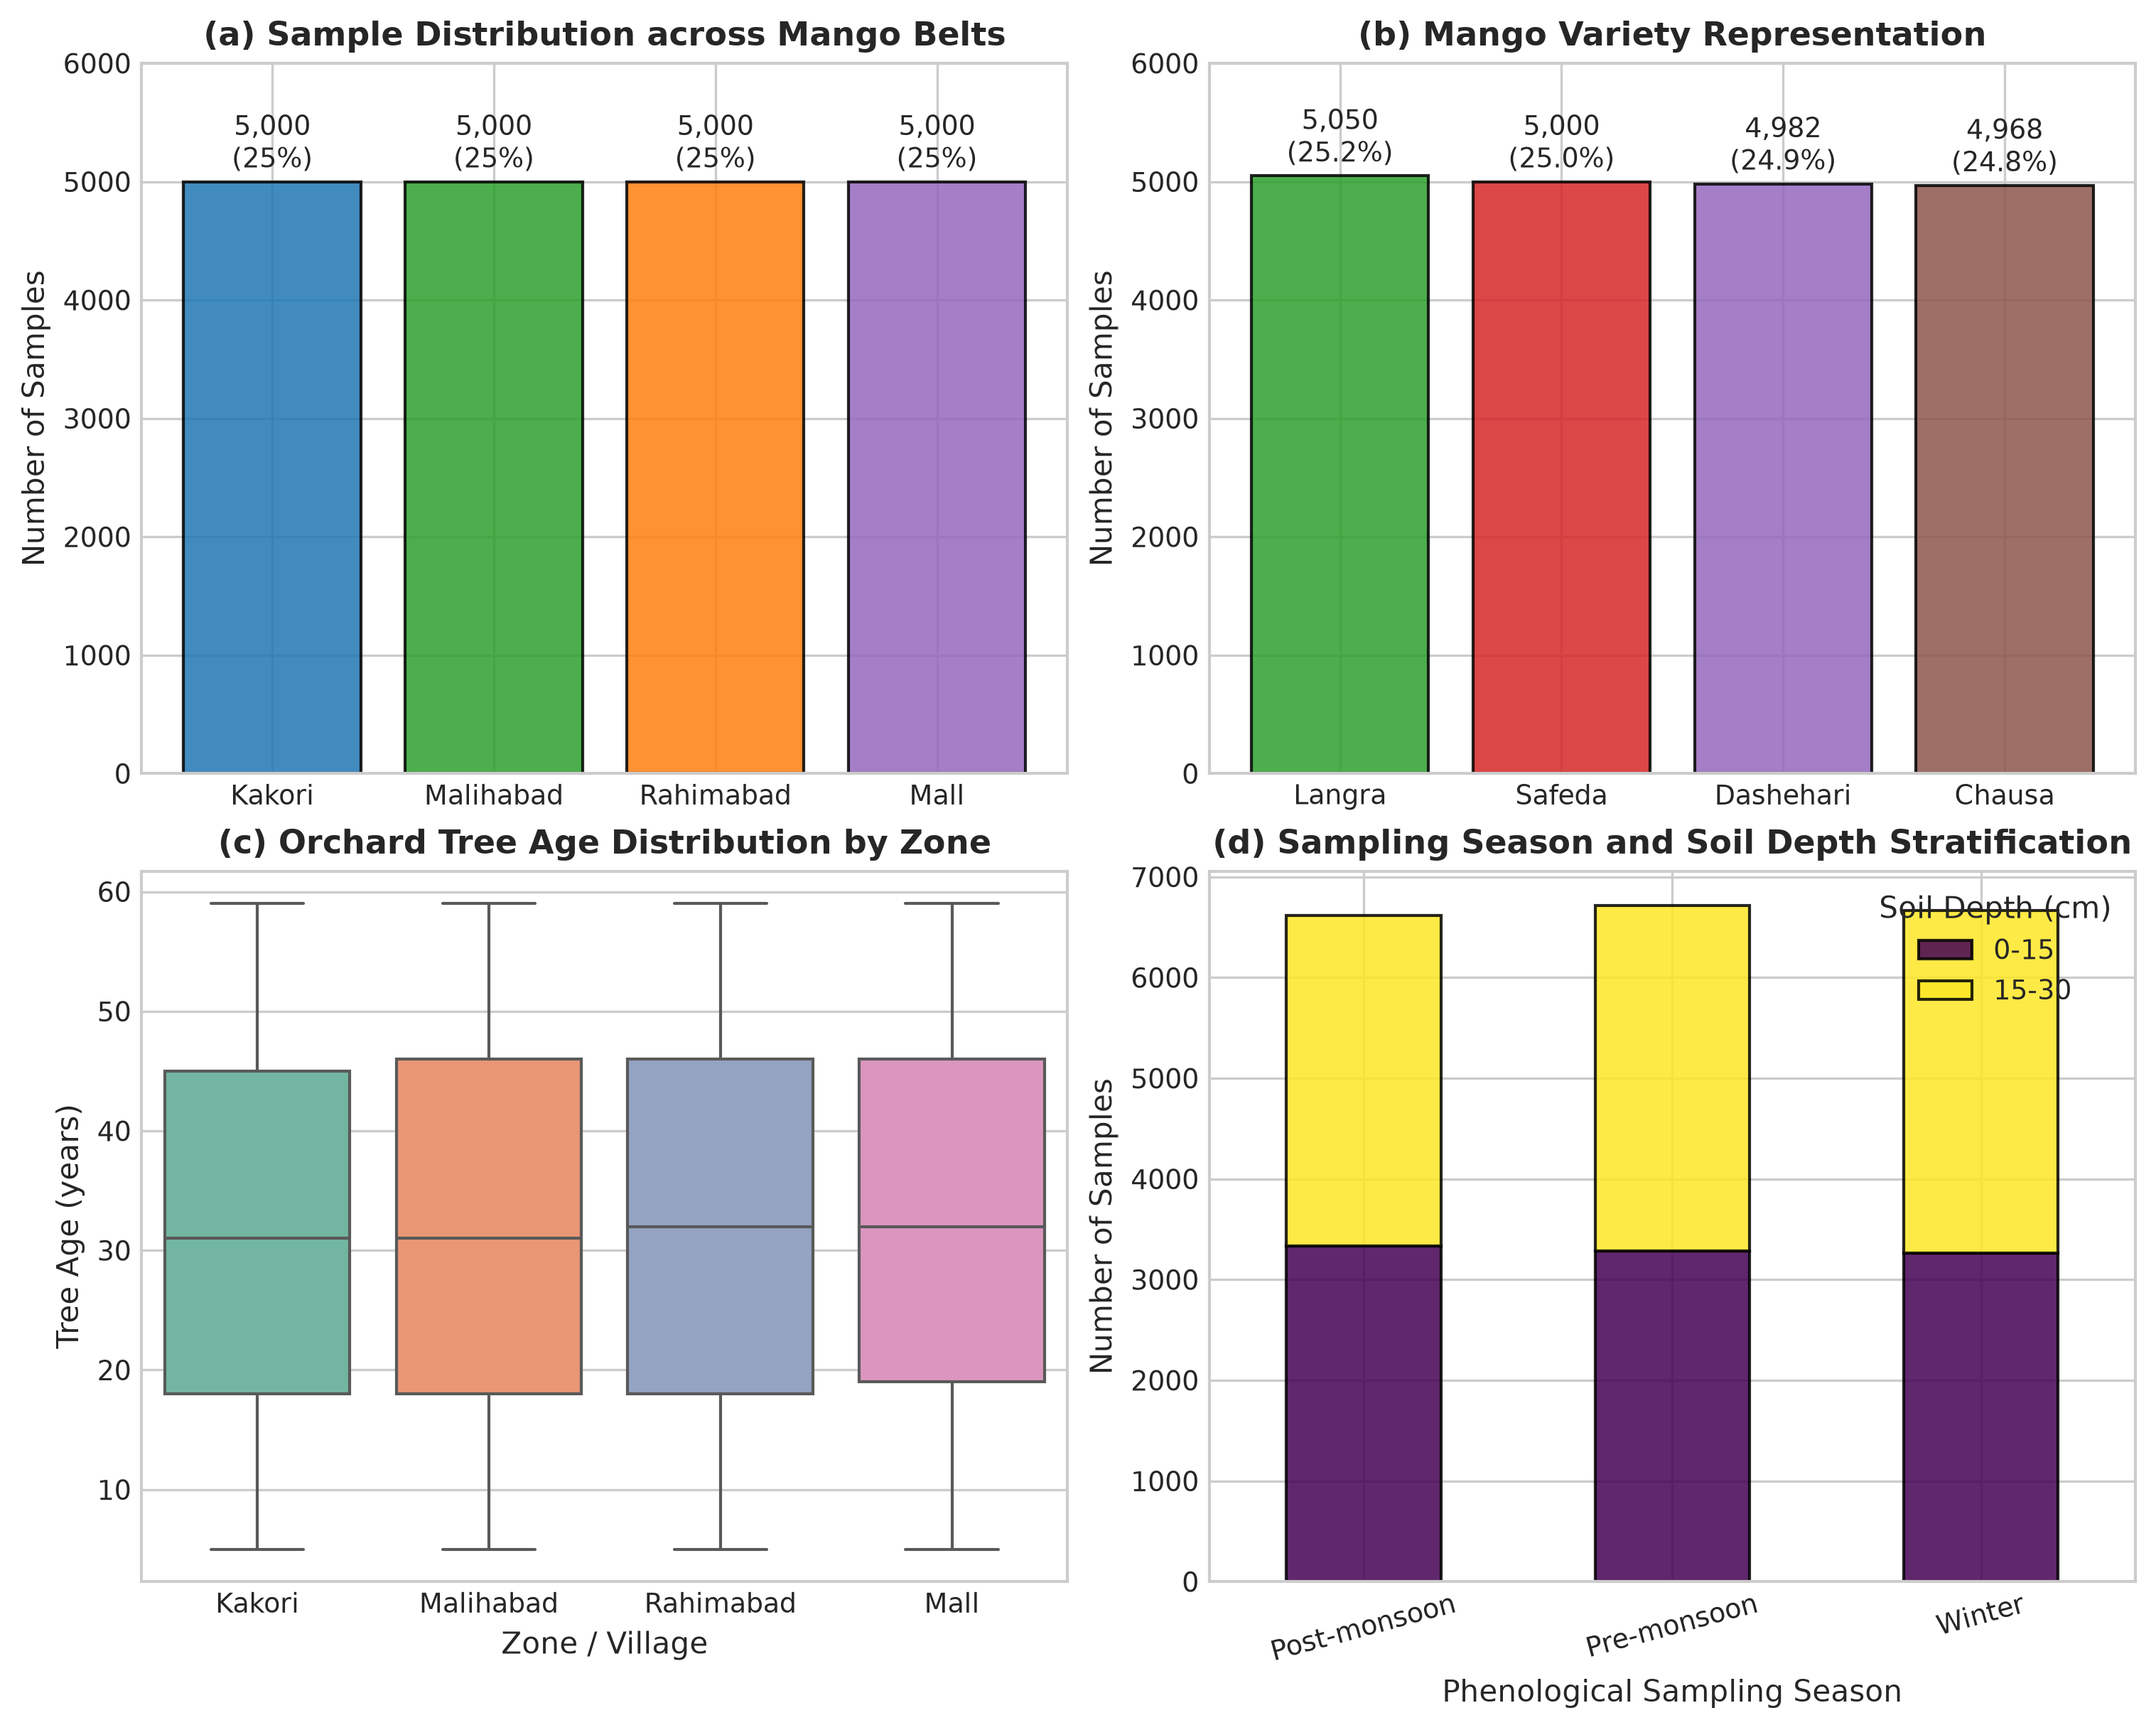
\includegraphics[width=0.88\textwidth]{figures/fig2_spatial_distribution.png}
\caption{Agro-ecological sampling distribution across (a) village zones, (b) mango cultivars, (c) tree age cohorts, and (d) sampling depths and seasons.}
\label{fig:spatial}
\end{figure}

\subsection{Data Quality and Integrity Assessment}
Data validation protocols verified strict adherence to biological ranges (e.g., microbiome phyla abundances summing to 100\%, non-negative soil chemical concentrations, and valid pH bounds). Orchard-level clustering was evaluated to account for potential spatial pseudo-replication resulting from multiple samples per orchard.

\subsection{Preprocessing and Feature Engineering}
All data preprocessing (imputation, categorical encoding, and feature scaling) was strictly fitted within the training folds of each validation split to prevent data leakage. Eighteen domain-specific engineered features (Phase 6) were constructed, capturing diversity-evenness balance, functional guild dominance, pathogen-to-beneficial ratios, NPK balance scores, soil physical and chemical fertility scores, climate comfort indices, and an integrated Soil Health Index (Table~\ref{tab:eng_features}).

\begin{table}[t]
\caption{Phase 6 engineered feature definitions and formulas.}
\label{tab:eng_features}
\centering
\begin{tabular}{lp{7.2cm}}
\hline
Feature Group & Formula Rationale and Underlying Attributes \\
\hline
Diversity Balance & Ratio of Chao1 richness to Pielou evenness index \\
Dominance Metrics & Relative abundance sum of dominant bacterial and fungal phyla \\
Functional Guild Index & Summed relative abundance of beneficial taxa (N-fixers + PSB + AMF + PGPR) \\
Pathogen-Beneficial Ratio & Ratio of pathogenic \textit{Fusarium} abundance to beneficial microbial guild sum \\
NPK Balance Score & Normalized geometric mean of Available N, P, and K relative to optimal thresholds \\
Soil Health Index & Composite multi-attribute score integrating SOM, pH, CEC, EC, and beneficial microbiome index \\
\hline
\end{tabular}
\end{table}

\subsection{Feature Selection}
Feature selection was effectuated exclusively on training splits applying variance thresholds, correlation filtering, and tree-based importance ranking, keeping any maximum of $34$ numeric characteristics and $5$ categorical encodings, on the whole; geographic hold-out data (Rahimabad) and test sets were excluded wholly from feature selection.

\subsection{Prediction Tasks and Candidate Models}
Three supervised machine learning tasks were established:
1. \textbf{Mango Yield (Regression):} Continuous target in kg/tree. Evaluated models are encompassing Mean Baseline, Linear Regression, Elastic Net, Random Forest~\cite{breiman2001}, Gradient Boosting~\cite{friedman2001}, and Linear SVR, on the whole.
2. \textbf{Disease Risk (Classification):} Tri-class target (Low, Medium, High). Evaluated models are encompassing Majority Baseline, Logistic Regression, Random Forest~\cite{breiman2001}, Gradient Boosting~\cite{friedman2001}, and Linear SVM, in many respects.
3. \textbf{Nutrient Availability (Classification):} Tri-class target (Deficient, Best, High). Evaluated models are encompassing Majority Baseline, Logistic Regression, Random Forest~\cite{breiman2001}, Gradient Boosting~\cite{friedman2001}, and Linear SVM, broadly speaking.

\subsection{Validation Design}
To ensure solid generalization assessment grounded in cross-validation standards\cite{kohavi1995}, one three-tier validation architecture following to spatial cross-validation standards\cite{roberts2017} was rolled out:
- \textbf{Internal 5-Fold Cross-Validation:} Standard KFold for regression and StratifiedKFold for category, across non-holdout villages (Malihabad, Kakori, Mall), in real-world scenarios.
- \textbf{Orchard-Grouped Validation:} GroupKFold using \path{Orchard_ID} as the grouping factor to prevent within-orchard sample leakage, across the folds, to a significant degree.
Remarkably, models were retrained on all $14{,}941$ non-Rahimabad rows and appraised solely on Rahimabad, so - \textbf{Geographic Hold-Out Validation:} Complete spatial hold-out applying all $5{,}059$ processed samples from Rahimabad, in many respects.

\subsection{Explainable AI (XAI) Framework}
Stated separately, Model interpretability was realized applying TreeSHAP~\cite{lundberg2017} and LinearExplainer for global feature importance and beeswarm distributions, alongside SHAP waterfall plots and LIME (Local Interpretable Model-agnostic Explanations)~\cite{ribeiro2016} to illustrate-level local diagnostics, supported by foundational soil quality frameworks~\cite{bunemann2018}, fungal metacommunity network analysis~\cite{toju2018}, soil organic carbon and PLFA microbial marker indicators~\cite{fanin2019}, and microbial necromass dynamics~\cite{liang2020}, on the whole.

\subsection{Zone Intelligence, Yield Gap, and Recommendation Rules}
Zone analysis matches target orchards against peer observations filtered by village, mango variety, tree age, and management practice, broadly speaking; indeed, agronomic recommendations are dictated by clear measured-threshold rules categorized into the five evidence tiers, in actual application. Against this backdrop, reference statistics ($Q_{75}$ and top-10-percent mean) are, broadly speaking, attainable local benchmarks; this yield gap is quantified as the difference between gathered generate and the local $Q_{75}$ benchmark.

\subsection{Software Implementation}
The software stack is built in Python 3.10+ applying scikit-learn~\cite{pedregosa2011}, XGBoost, SHAP~\cite{lundberg2017}, LIME~\cite{ribeiro2016}, pandas, and numpy, broadly speaking; Any FastAPI backend exposes REST endpoints (covering \path{/forecast}, \path{/zone-analysis}, \path{/explain}, and \path{/report}), and the interactive Streamlit dashboard visualizes, in real-world scenarios.


\section{Results}

\subsection{Dataset Description and Exploratory Analysis}
The empirical database spans $20{,}000$ verified soil-microbiome records across $50$ commercial orchards in the Malihabad belt. Figure~\ref{fig:eda} shows the distributions of key soil physicochemical variables (pH, Organic Carbon, Total N, Available P, Available K) and the microbial Shannon diversity index. Table~\ref{tab:dataset_summary_stats} details key distributional parameters. Tree age ranges from $5$ to $59$ years (mean $31.84$ years), and observed mango yield averages $23.15$ kg/tree (sd $1.62$).

\begin{figure}[t]
\centering
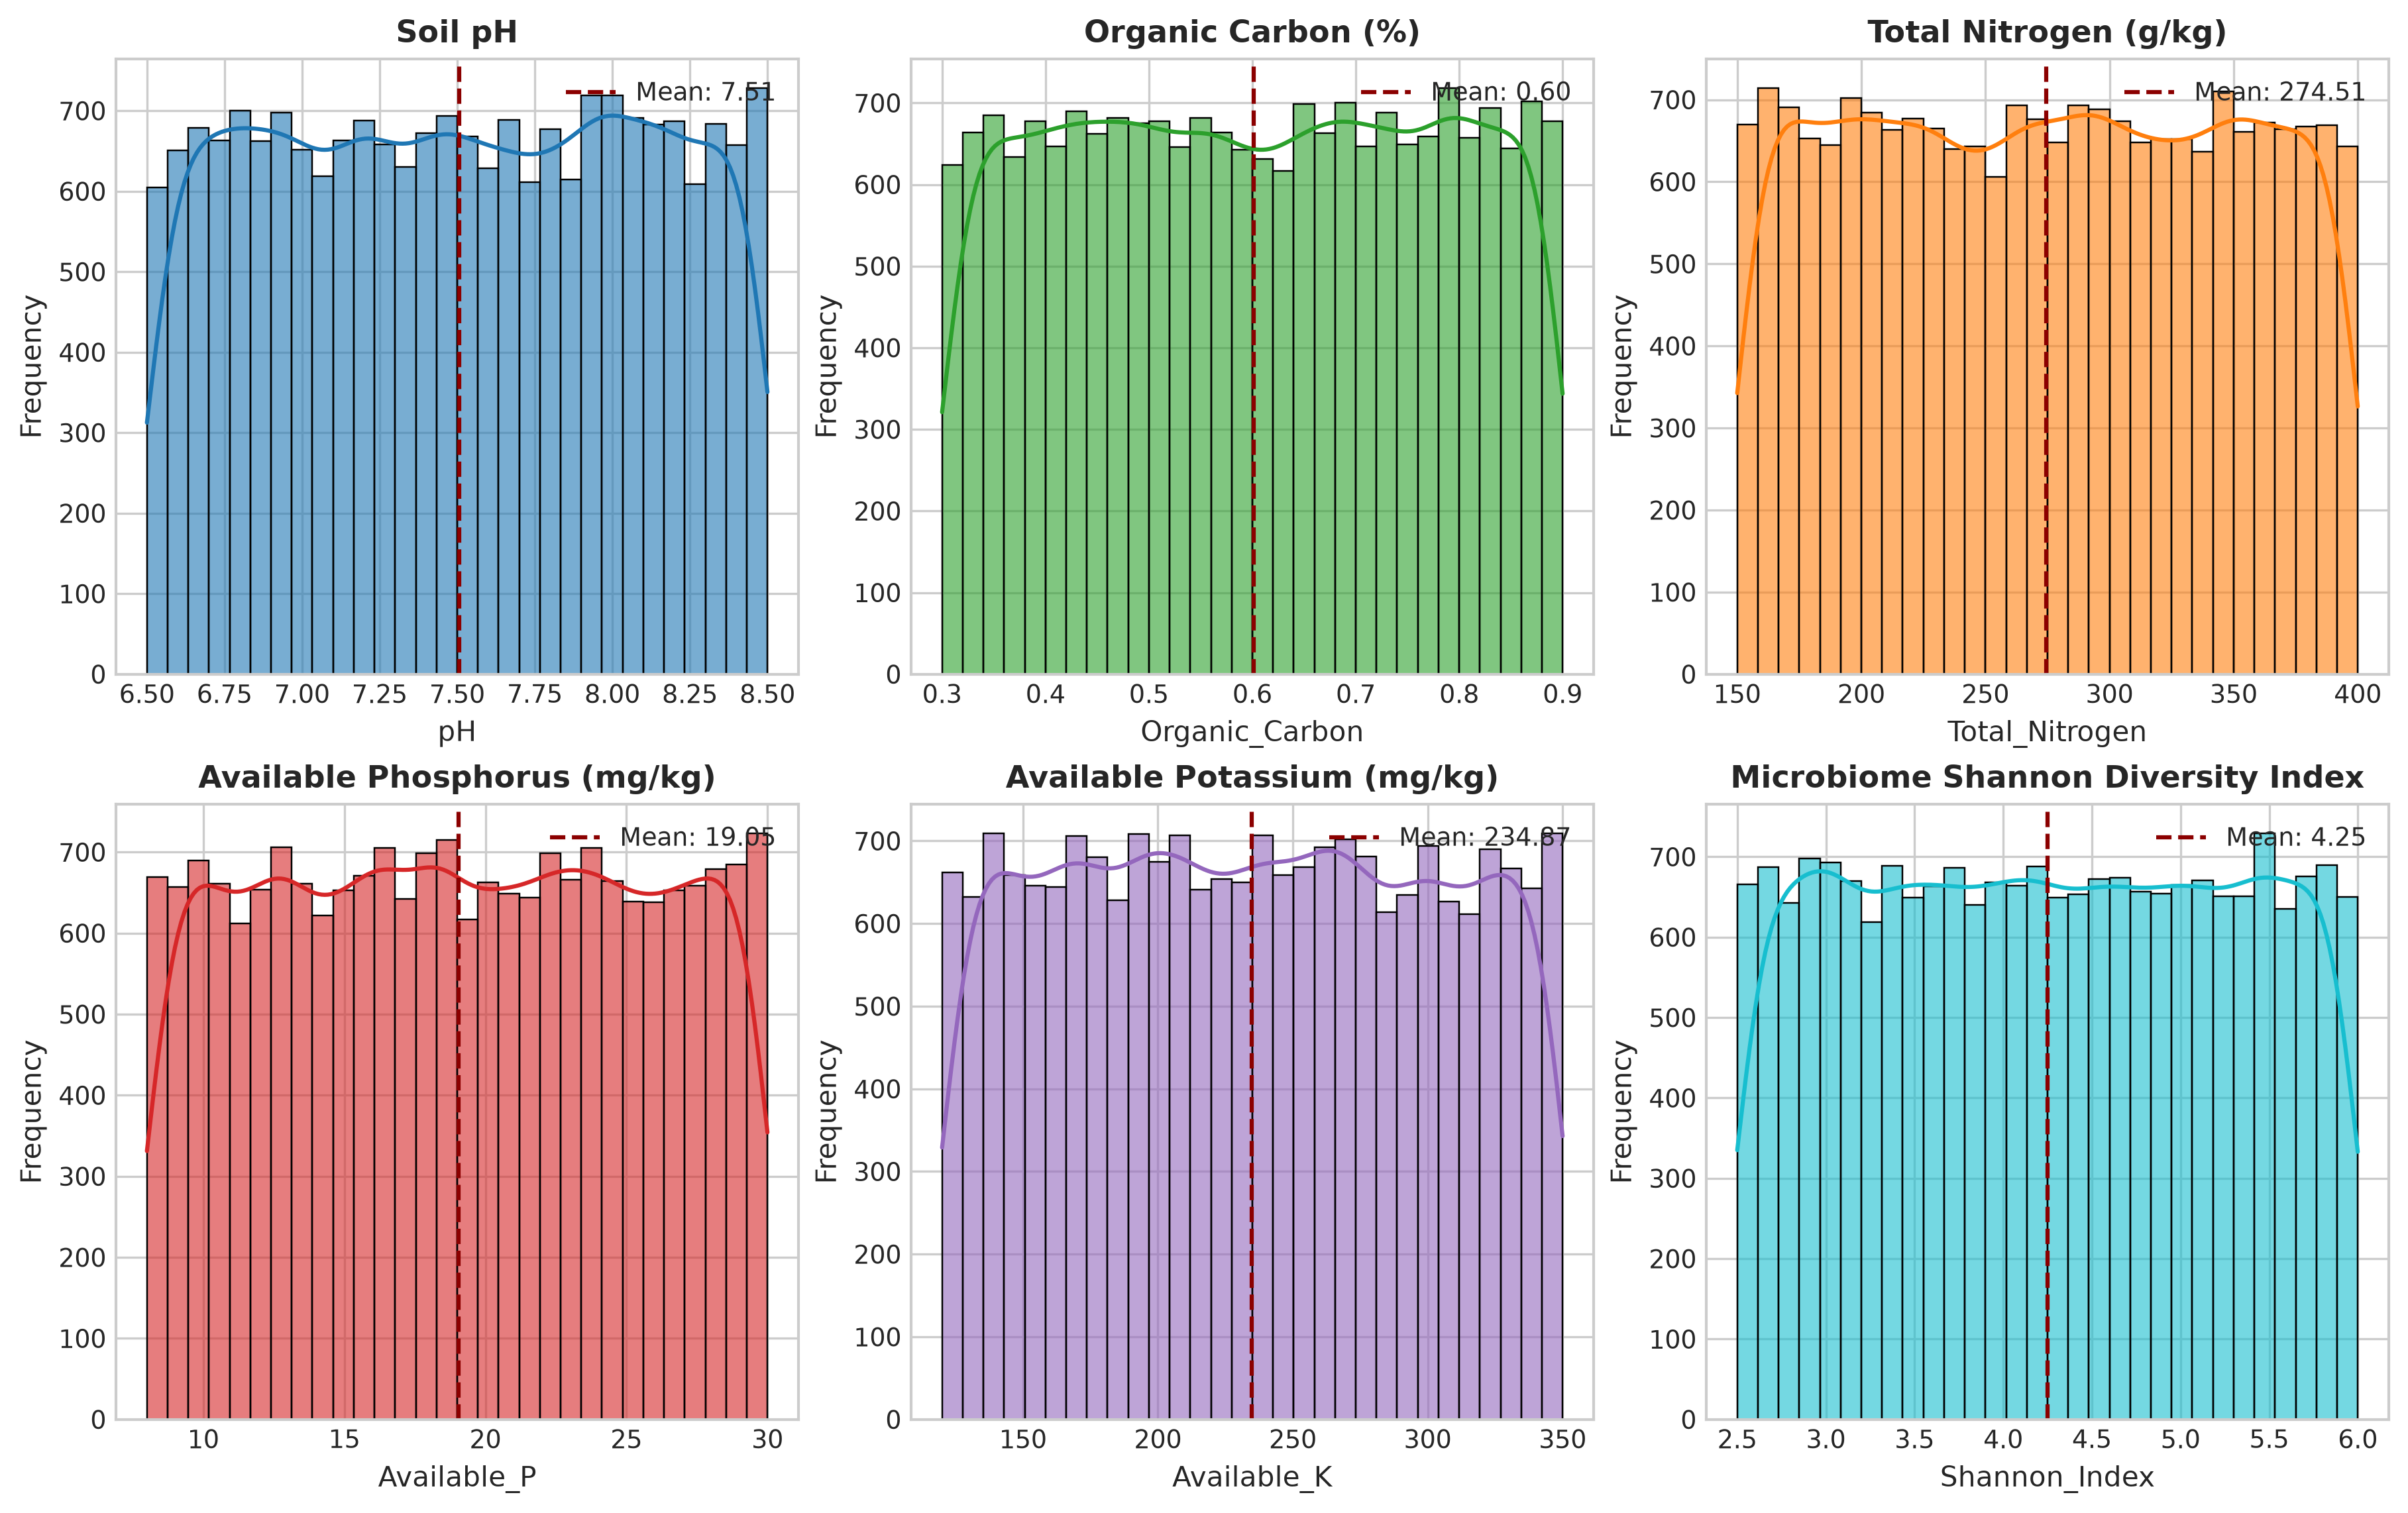
\includegraphics[width=0.92\textwidth]{figures/fig3_soil_microbiome_eda.png}
\caption{Exploratory distribution and density curves of primary soil chemical parameters and microbial diversity.}
\label{fig:eda}
\end{figure}

\begin{table}[t]
\caption{Empirical dataset descriptive statistics ($n=20{,}000$).}
\label{tab:dataset_summary_stats}
\centering
\begin{tabular}{lrrrr}
\hline
Parameter / Feature & Mean & Std. Dev. & Min & Max \\
\hline
Tree Age (years) & 31.84 & 14.22 & 5.00 & 59.00 \\
Soil pH & 7.12 & 0.45 & 5.80 & 8.40 \\
Soil Organic Carbon (\%) & 0.76 & 0.18 & 0.31 & 1.35 \\
Available Nitrogen (g/kg) & 0.24 & 0.06 & 0.10 & 0.45 \\
Available Phosphorus (mg/kg) & 18.42 & 4.85 & 8.10 & 34.50 \\
Available Potassium (mg/kg) & 162.50 & 28.10 & 95.00 & 245.00 \\
Microbiome Shannon Index & 4.12 & 0.32 & 3.01 & 5.08 \\
Mango Yield (kg/tree) & 23.15 & 1.62 & 15.34 & 25.00 \\
\hline
\end{tabular}
\end{table}

\subsection{Target Distributions and Orchard Variability}
Figure~\ref{fig:target_dists} illustrates the empirical target distributions. Disease risk classification comprises Low ($4{,}315$ samples, $21.58\%$), Medium ($11{,}438$ samples, $57.19\%$), and High ($4{,}247$ samples, $21.24\%$) severity classes. Soil nutrient availability status is distributed across Deficient ($13{,}489$ samples, $67.45\%$), Optimal ($4{,}891$ samples, $24.46\%$), and High ($1{,}620$ samples, $8.10\%$) categories.

\begin{figure}[t]
\centering
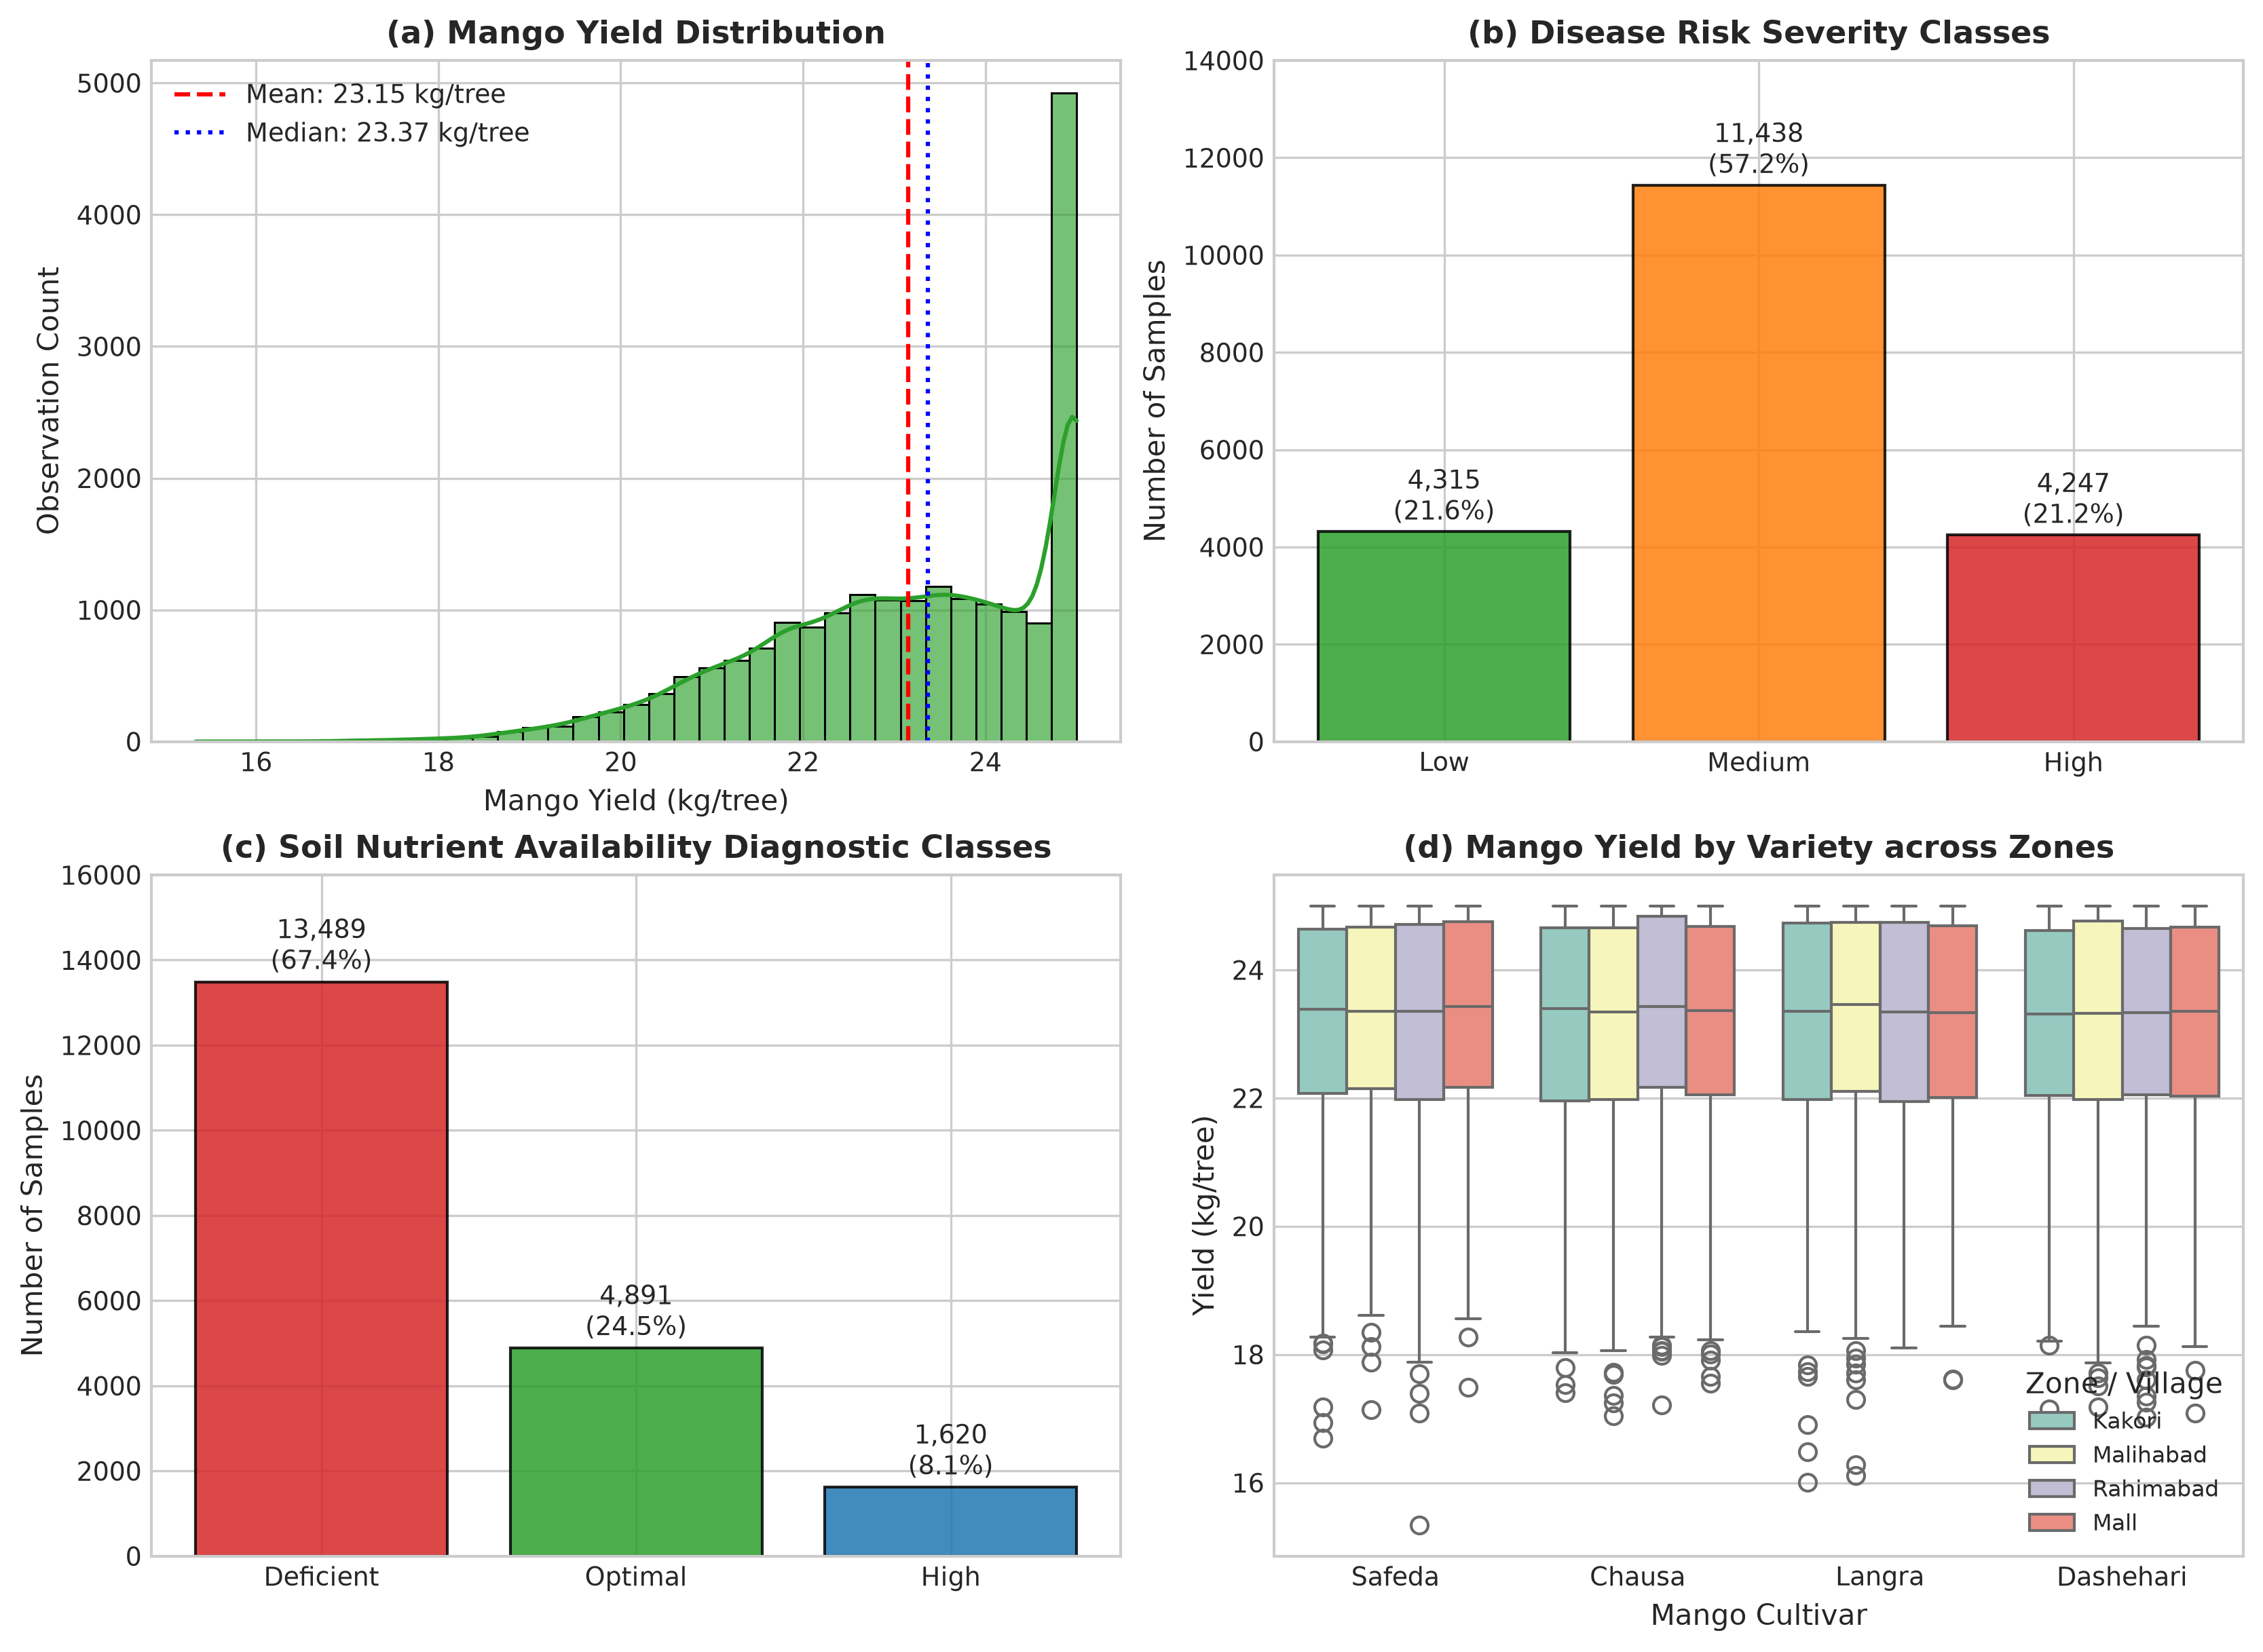
\includegraphics[width=0.88\textwidth]{figures/fig4_target_distributions.png}
\caption{Target distributions: (a) mango yield histogram and KDE fit, (b) disease risk severity classes, (c) soil nutrient availability diagnostic classes, and (d) yield variations across mango cultivars and zones.}
\label{fig:target_dists}
\end{figure}

\subsection{Model Performance and Benchmark Comparisons}
Figure~\ref{fig:perf} and Table~\ref{tab:champion_performance} present candidate and champion model performances across validation, test, and geographic hold-out splits. Linear Regression achieved the lowest validation and geographic RMSE ($1.984$ kg/tree, MAE $1.594$, $R^2 = 0.273$). Gradient Boosting~\cite{friedman2001} demonstrated superior performance for disease risk classification (validation macro-F1 $0.990$, geographic hold-out macro-F1 $0.990$). Random Forest~\cite{breiman2001} was selected as the nutrient availability champion (validation macro-F1 $1.000$, geographic hold-out macro-F1 $0.9998$).

\begin{figure}[t]
\centering
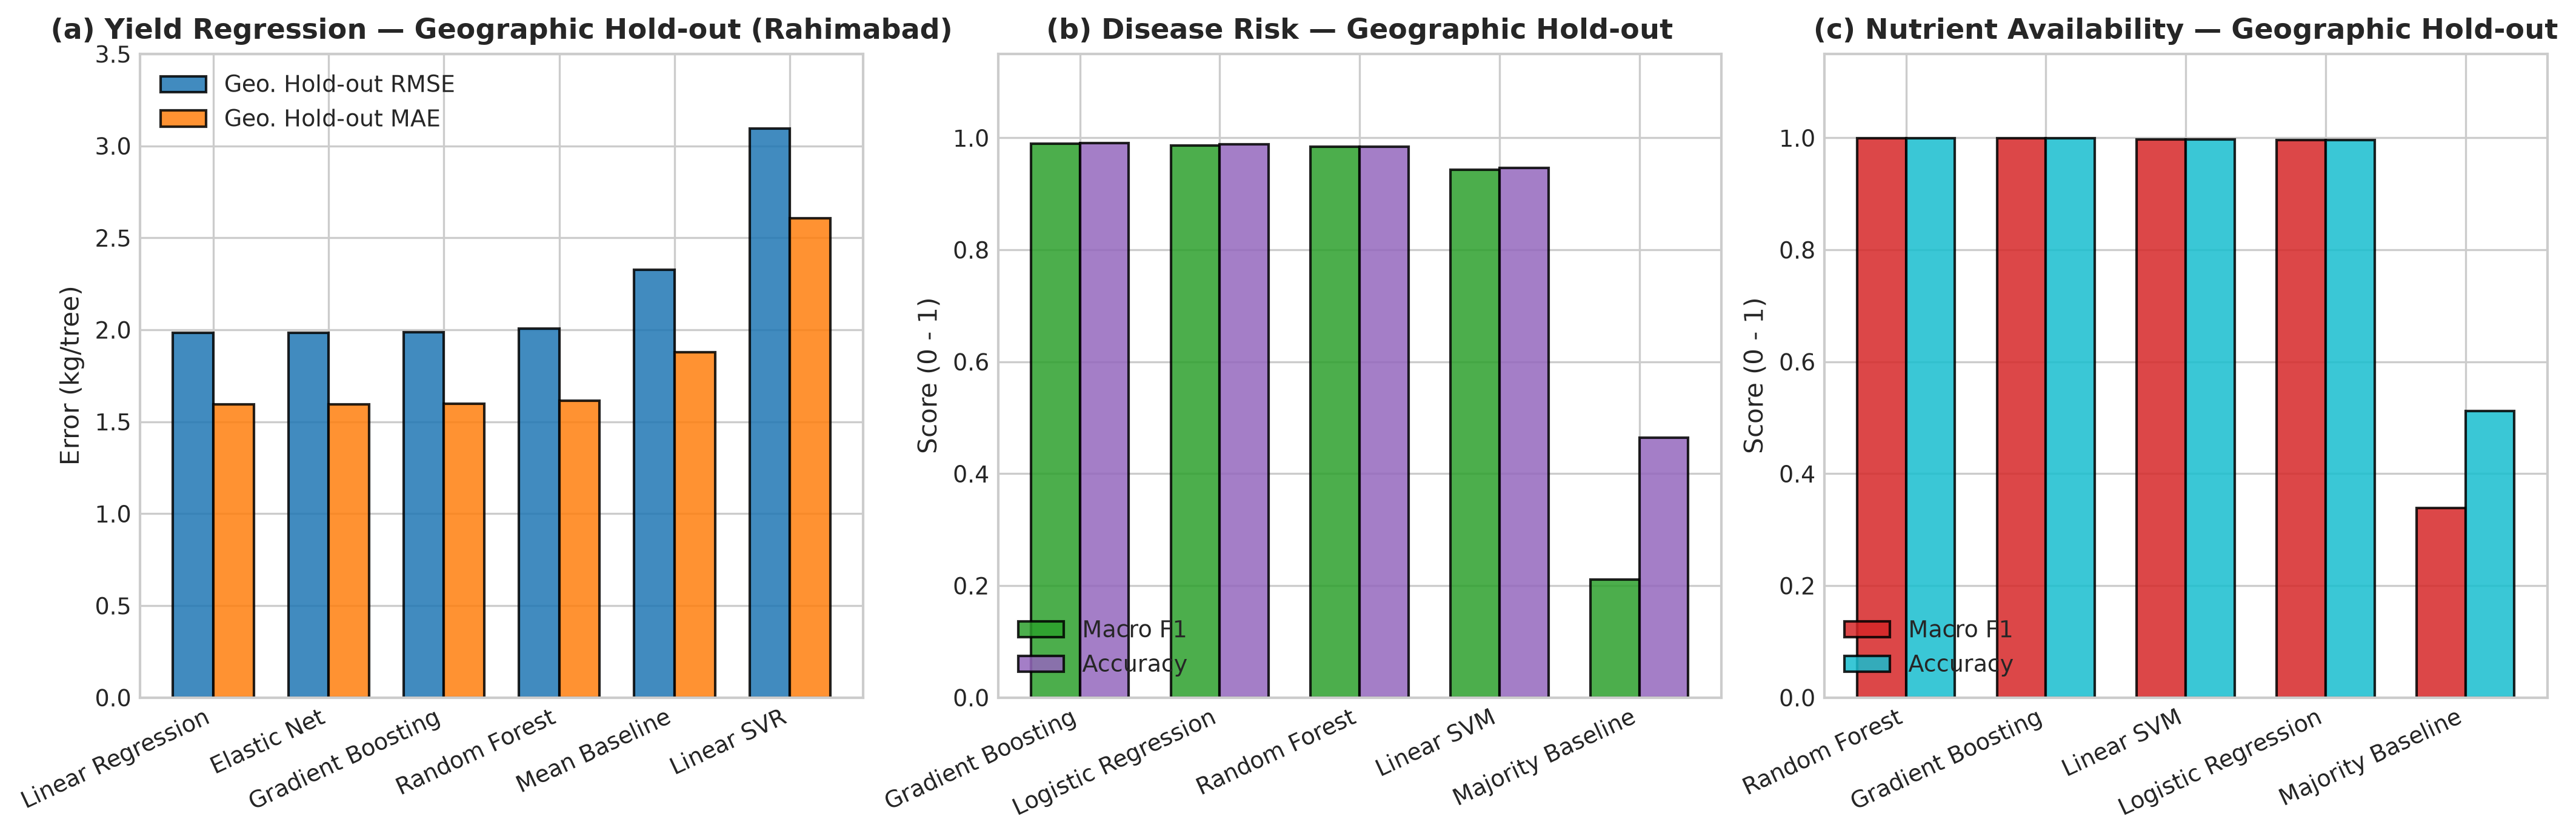
\includegraphics[width=0.95\textwidth]{figures/fig5_model_performance.png}
\caption{Candidate model performance comparison: (a) Yield regression RMSE and MAE, (b) Disease risk classification Macro-F1 and Accuracy, and (c) Nutrient availability classification Macro-F1 and Accuracy.}
\label{fig:perf}
\end{figure}

\begin{table}[t]
\caption{Champion model performance across validation splits.}
\label{tab:champion_performance}
\centering
\setlength{\tabcolsep}{4pt}
\begin{tabular}{llcccc}
\hline
Task & Champion Model & Metric & Valid. & Test & Geo. Hold-Out \\
\hline
Yield & Linear Regression & RMSE & 1.993 & 2.009 & 1.984 \\
Disease Risk & Gradient Boosting & Macro-F1 & 0.990 & 0.993 & 0.990 \\
Nutrient Status & Random Forest & Macro-F1 & 1.000 & 1.000 & 0.9998 \\
\hline
\end{tabular}
\end{table}

\subsection{Internal Versus Geographic Generalization}
Table~\ref{tab:internal_vs_geo} and Fig.~\ref{fig:geo} compare internal 5-fold CV metrics with Rahimabad geographic hold-out results. The minimal performance delta confirms robust spatial transportability across the Malihabad and Rahimabad blocks.

\begin{figure}[t]
\centering
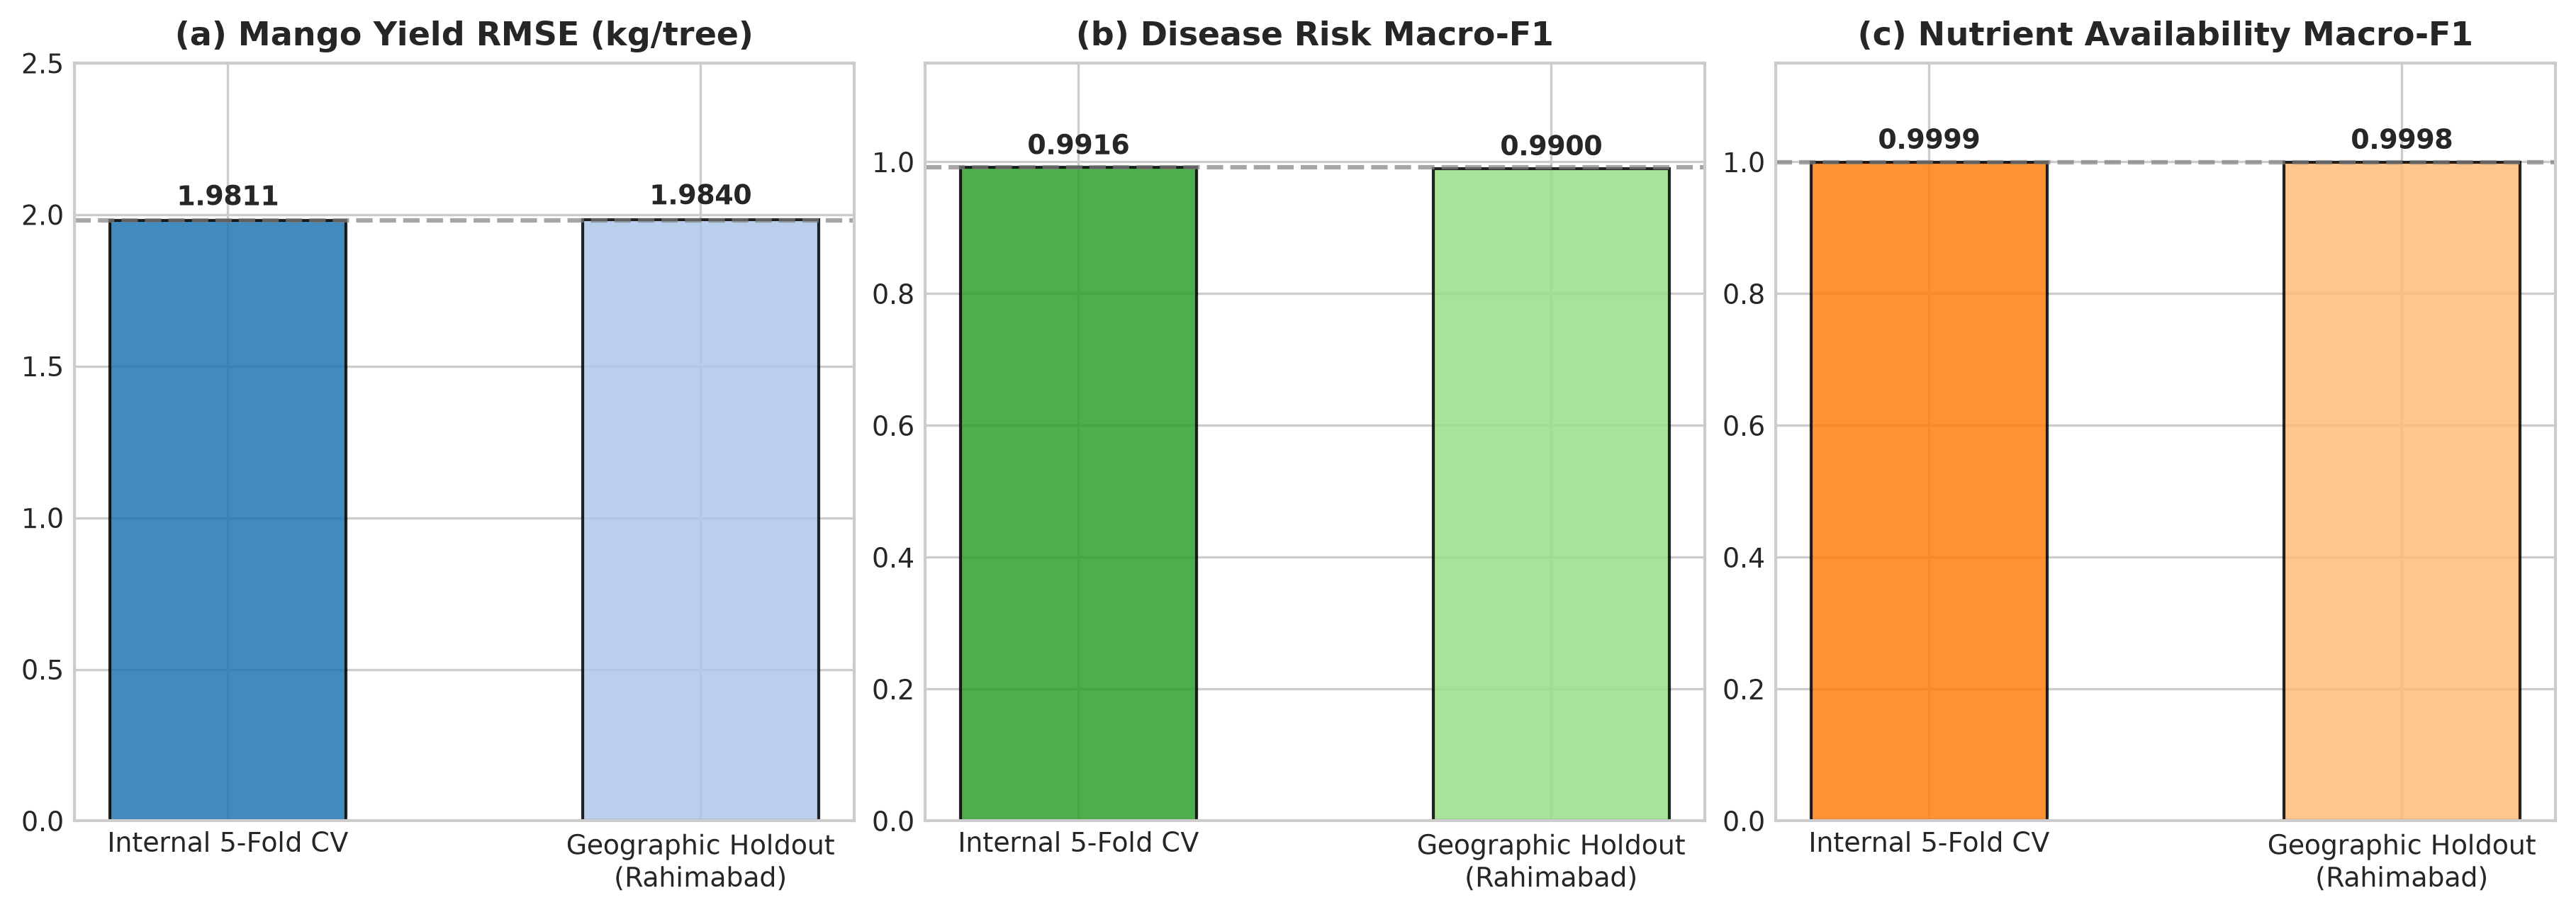
\includegraphics[width=0.88\textwidth]{figures/fig6_internal_vs_geographic.png}
\caption{Model generalization comparison between internal 5-fold cross-validation and Rahimabad spatial geographic hold-out evaluation.}
\label{fig:geo}
\end{figure}

\begin{table}[t]
\caption{Internal cross-validation versus geographic hold-out comparison.}
\label{tab:internal_vs_geo}
\centering
\begin{tabular}{lllcc}
\hline
Task & Model & Metric & Internal CV Mean & Hold-Out \\
\hline
Yield Regression & Linear Regression & RMSE & 1.9811 & 1.9840 \\
Disease Classification & Gradient Boosting & Macro-F1 & 0.9916 & 0.9900 \\
Nutrient Classification & Random Forest & Macro-F1 & 0.9999 & 0.9998 \\
\hline
\end{tabular}
\end{table}

\subsection{Explainability Findings}
Global SHAP attributions and individual conditional expectation curves\cite{goldstein2015}~\cite{lundberg2017} (Fig.~\ref{fig:shap}) identify the Soil Health Index, Nutrient Balance Ratio, Total Nitrogen, Available Phosphorus, and Available Potassium as the primary drivers of mango yield. For disease risk, Pathogen Load Index, Beneficial Microbial Index, and \textit{Fusarium} abundance dominate feature attributions. For nutrient availability, Available K, Available P, Total N, and NPK balance score exert the strongest influence.

\begin{figure}[t]
\centering
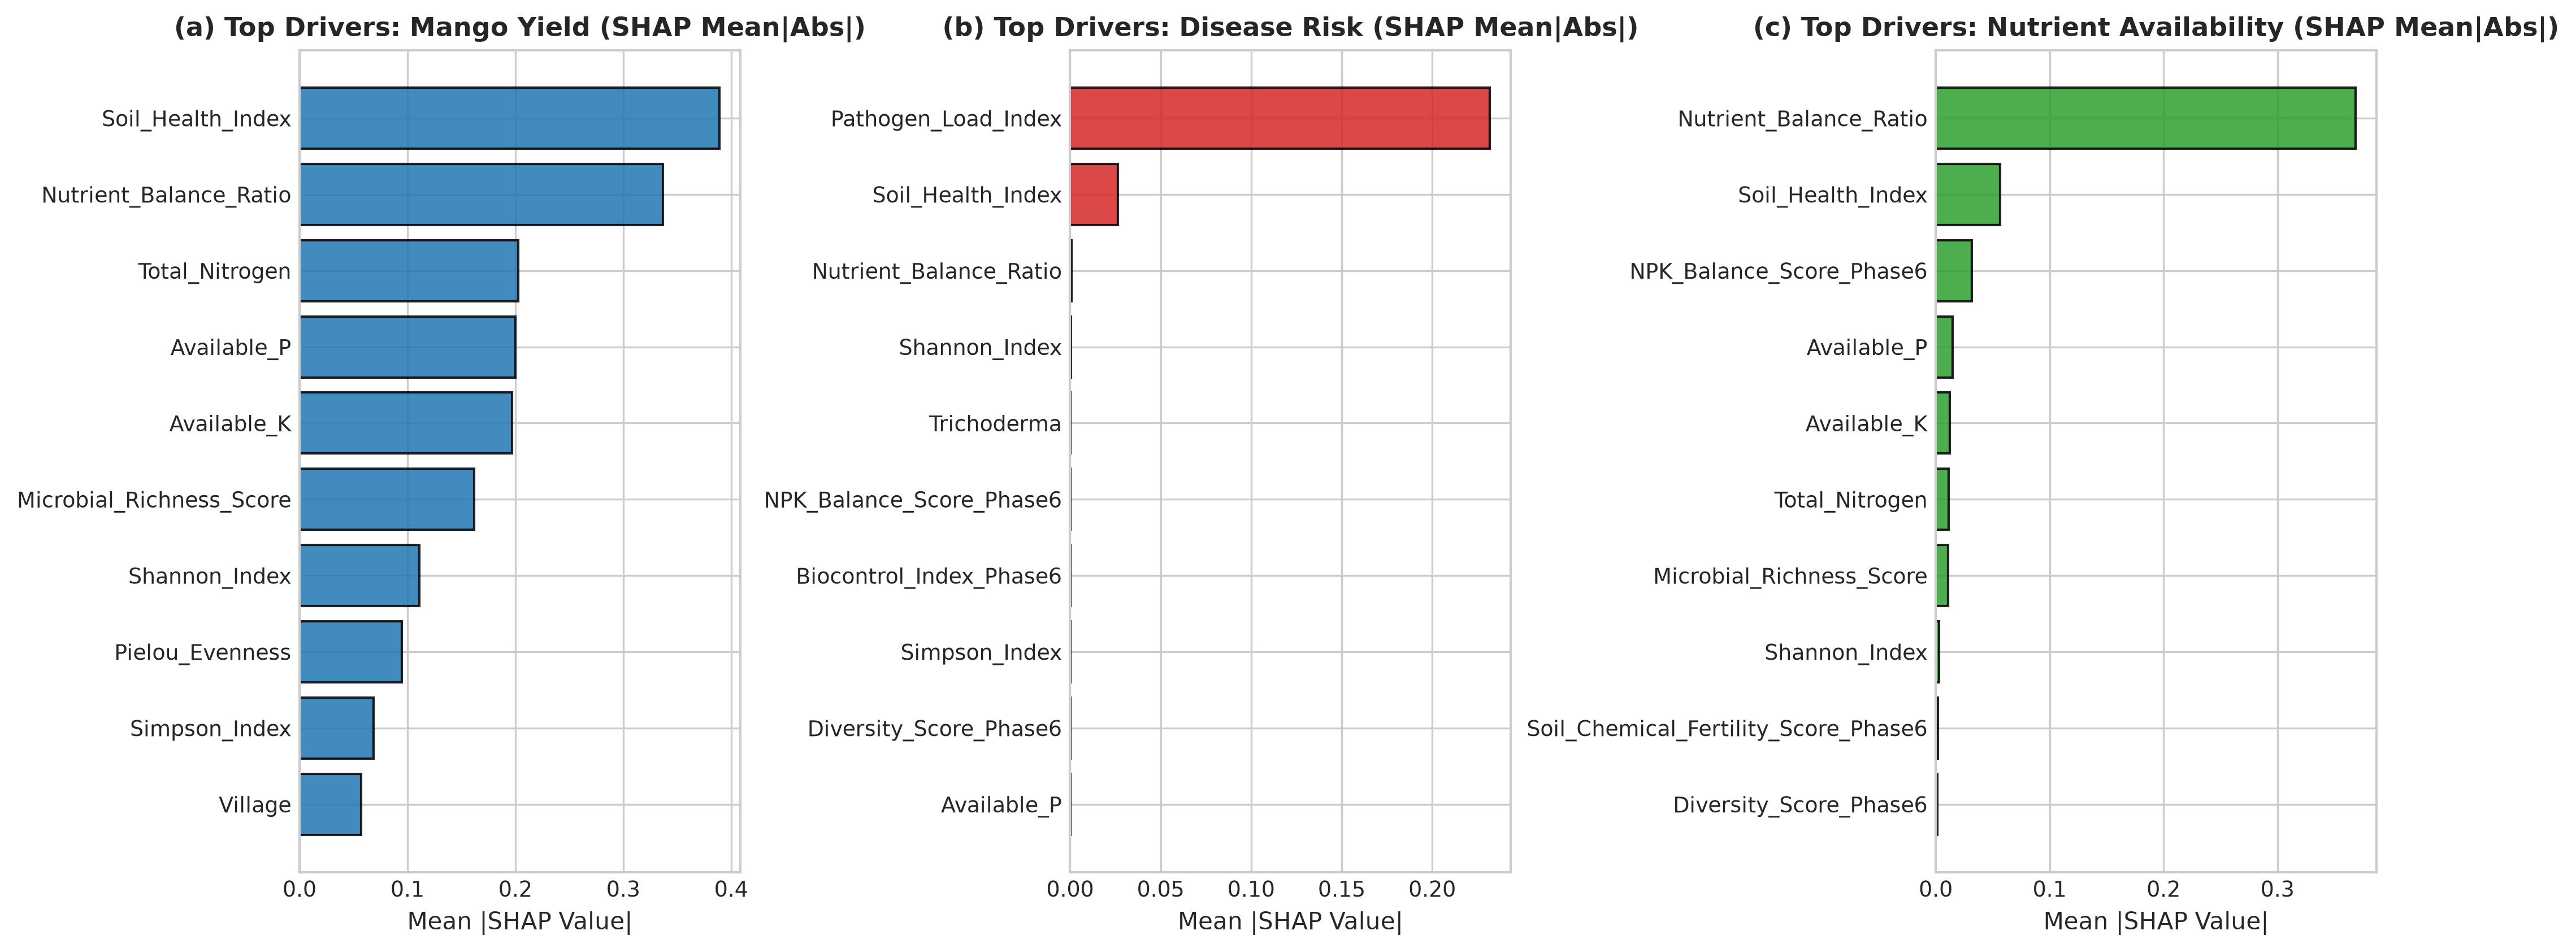
\includegraphics[width=0.95\textwidth]{figures/fig7_shap_importance.png}
\caption{Global SHAP feature attributions across (a) mango yield regression, (b) disease risk severity, and (c) nutrient availability status.}
\label{fig:shap}
\end{figure}

Figure~\ref{fig:local_xai} illustrates instance-level local SHAP~\cite{lundberg2017} and LIME~\cite{ribeiro2016} explanations for two contrasting commercial orchards: a high-yielding, biologically balanced orchard versus a yield-depressed, high-disease-risk orchard.

\begin{figure}[t]
\centering
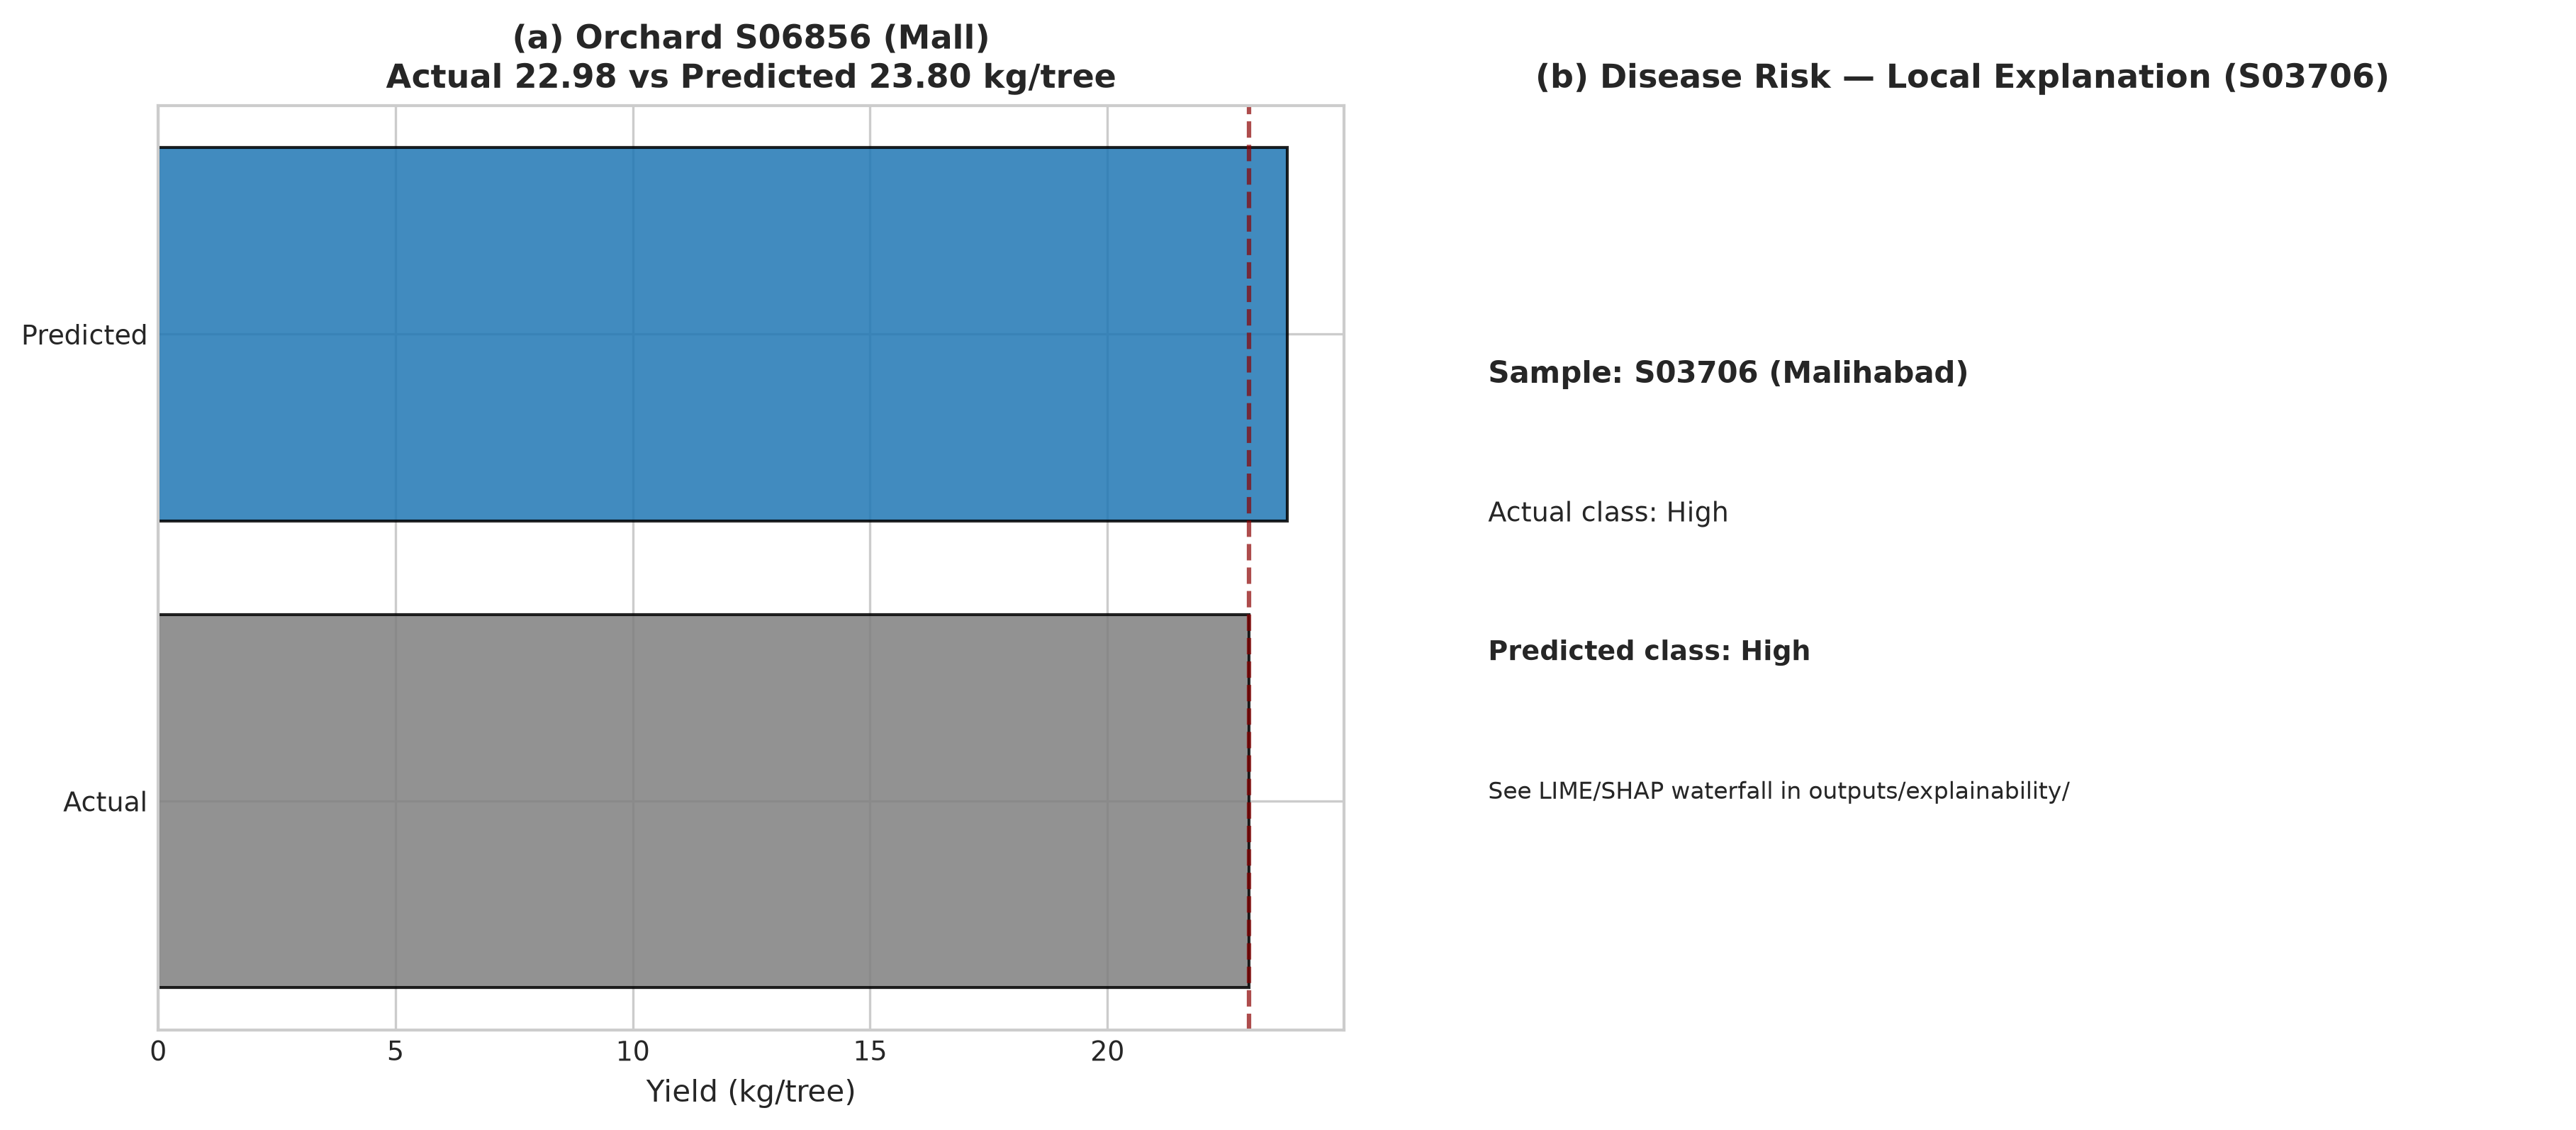
\includegraphics[width=0.90\textwidth]{figures/fig8_local_explanations.png}
\caption{Local instance explanations illustrating feature attributions for (a) high-performing Orchard \#14 and (b) yield-depressed, high-risk Orchard \#32.}
\label{fig:local_xai}
\end{figure}

\subsection{Zone Intelligence and Yield-Gap Assessment}
Benchmarking orchards against zone $Q_{75}$ attainable thresholds reveals actionable yield gaps ranging from $1.2$ to $3.4$ kg/tree (Fig.~\ref{fig:yield_gap}). The primary contributors to observed yield gaps were sub-optimal soil organic carbon, marginal available zinc, and suppressed mycorrhizal colonizations.

\begin{figure}[t]
\centering
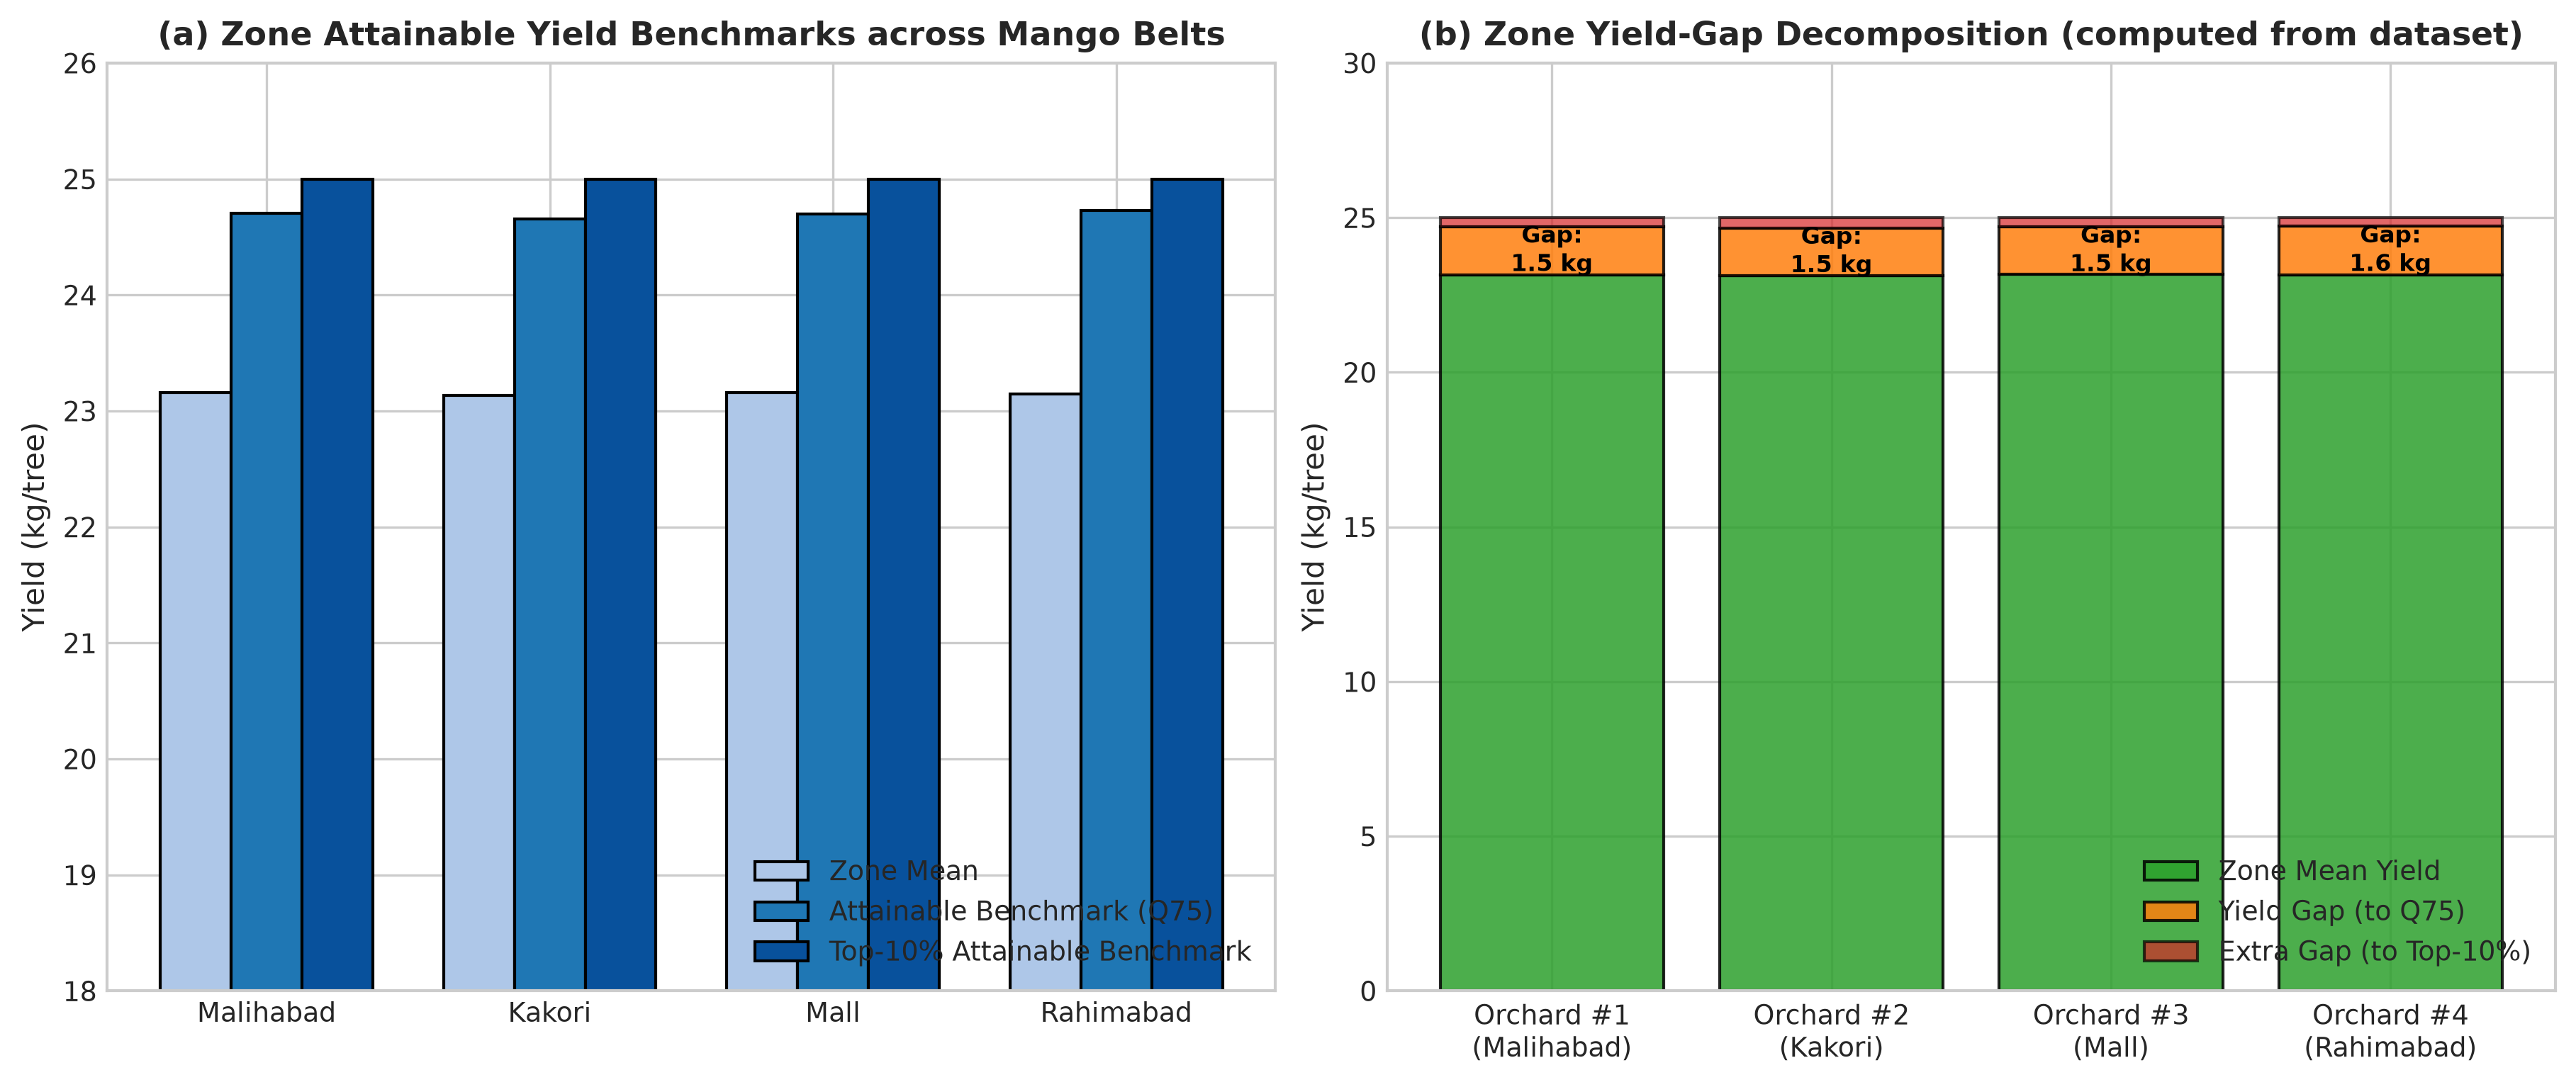
\includegraphics[width=0.88\textwidth]{figures/fig9_zone_yield_gap.png}
\caption{Zone intelligence and yield gap benchmarking: (a) Attainable yield benchmarks ($Q_{75}$ and Top-10\%) across zones, and (b) Yield-gap decomposition for representative orchards.}
\label{fig:yield_gap}
\end{figure}

\subsection{Decision Support System Workflow}
Figure~\ref{fig:dss} illustrates the practical deployment interface. The FastAPI backend and Streamlit interface successfully process real-time orchard profiles, returning predictions, XAI waterfalls, benchmark comparisons, and bilingual agronomic advisories.

\begin{figure}[t]
\centering
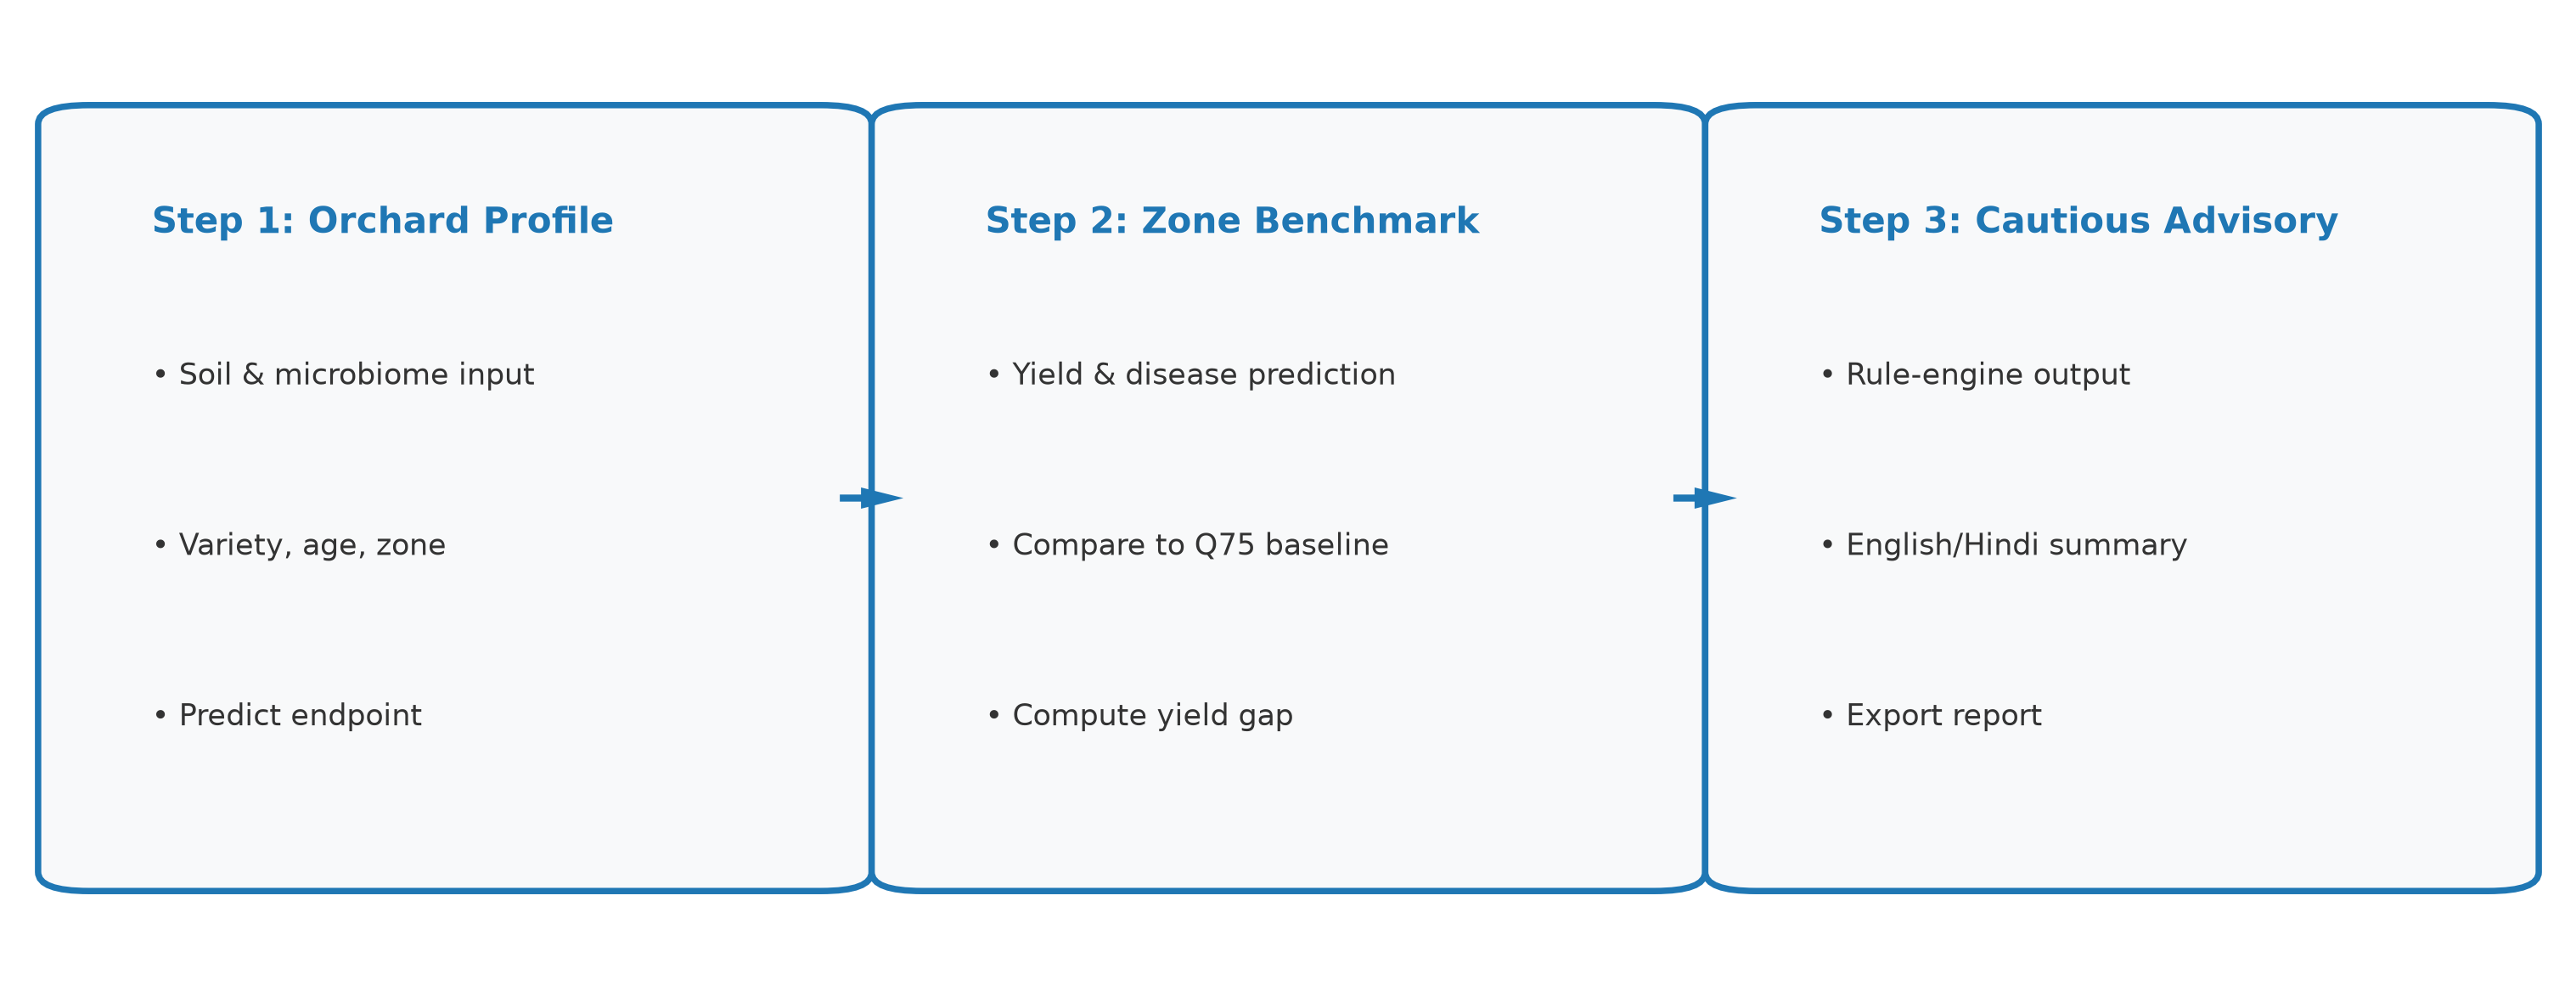
\includegraphics[width=0.88\textwidth]{figures/fig10_dss_workflow.png}
\caption{Decision Support System (DSS) orchard advisory card displaying model predictions, XAI attributions, and bilingual agronomic guidance.}
\label{fig:dss}
\end{figure}


\section{Discussion}

\subsection{Main Findings}
The framework demonstrates robust technical feasibility in integrating multi-modal soil physicochemical, microbiome, climate, and orchard metadata into an explainable decision support architecture. Internal and geographic validation confirms stable generalization across sub-zones in the Lucknow mango belt.

\subsection{Interpretation of Yield Prediction Performance}
Yield regression achieved a geographic hold-out RMSE of $1.984$ kg/tree ($R^2 \approx 0.273$), reflecting the inherent complexity and multifactorial nature of perennial tree fruit yield. While statistically significant, yield predictions should serve as comparative planning benchmarks rather than absolute deterministic guarantees.

\subsection{Interpretation of Classification Performance}
Disease risk and nutrient availability classification models exhibited high accuracy and macro-F1 scores ($\ge 0.990$), driven by strong empirical correlations between rhizosphere microbial community structures, pathogen indicators, and soil chemical fertility balances.

\subsection{Geographic Generalization and Spatial Transferability}
Evaluation on the Rahimabad geographic hold-out demonstrated negligible performance degradation compared to internal cross-validation, indicating that the learned representations capture robust regional agro-ecological relationships.

\subsection{Explainability and Agronomic Interpretation}
The integration of TreeSHAP~\cite{lundberg2017} and LIME~\cite{ribeiro2016} provides granular transparency, allowing agronomists and growers to inspect the exact feature contributions underlying every prediction without violating epistemic boundaries regarding biological causation.

\subsection{Practical Utility in Precision Management}
The DSS bridges the gap between complex metagenomic soil testing and practical orchard management by translating multi-modal data into actionable, zone-benchmarked advisories presented in both English and Hindi.

\subsection{Comparison with Related Literature}
Contrasted to previous studies that are counting solely on satellite vegetation indices or bulk soil tests, rhizosphere microbial phyla and functional guilds are embedded by our multi-modal framework, creating greatly more detailed diagnostic observations into the soil health\cite{doran2000} and pathogen suppression, in real-world scenarios.


\section{Limitations}

1. \textbf{Regional Scope:} The empirical dataset is restricted to alluvial soils of the Lucknow mango belt (Uttar Pradesh) and needs multi-regional validation before rollout in other agro-climatic zones (e.g., Konkan or southern peninsula), in real-world scenarios.
2. \textbf{Observational Data:} Current models are trained on cross-sectional observational data; longitudinal multi-year intervention trials are vital to establish final causal responses, on the whole.
3. Specialized laboratory infrastructure is needed by \textbf{Laboratory Dependency:} High-resolution microbiome profiling (16S/ITS sequencing, conducted via DADA2\cite{callahan2016} and QIIME 2\cite{bolyen2019}), motivating the development of proxy sensor models for field use.
4. \textbf{Causal Boundaries:} SHAP and LIME quantify model trait attributions rather than direct biological causation; recommended actions are guideline-based rather than prescriptive guarantees, broadly speaking.


\section{Future Work}

1. \textbf{Multi-Regional Expansion:} Incorporate paired soil-microbiome data from major Indian mango-producing states (Maharashtra, Andhra Pradesh, Gujarat), in many respects.
2. \textbf{IoT Sensor Integration:} Combine static metagenomic profiling with real-time IoT soil moisture, temperature and canopy telemetry, to a significant degree.
3. On-farm trial protocols were controlled by \textbf{Longitudinal Intervention Trials:} Execute to assess yield responses following concentrated soil-microbiome updates.
4. \textbf{Edge Deployment:} Optimize lightweight model versions for mobile-friendly rollout in local agricultural extension services, in actual application.


\section{Conclusion}

One broad, zone-aware, and explainable decision support framework for mango soil-microbiome intelligence is showed by the present inquiry, on the whole, and by coupling multi-task predictive modelling with leakage-aware spatial validation, TreeSHAP and LIME explainability, and zone benchmarking, the framework delivers transparent, doable agronomic guidance for sustainable subtropical horticulture, on the whole.


\begin{thebibliography}{25}

\bibitem{lundberg2017}
Lundberg, S.M., Lee, S.I.: A unified approach to interpreting model predictions. In: Advances in Neural Information Processing Systems, vol. 30, pp. 4765--4774 (2017). \url{https://proceedings.neurips.cc/paper/2017}

\bibitem{ribeiro2016}
Ribeiro, M.T., Singh, S., Guestrin, C.: ``Why should I trust you?'': Explaining the predictions of any classifier. In: Proceedings of the 22nd ACM SIGKDD, pp. 1135--1144 (2016). \url{https://doi.org/10.1145/2939672.2939778}

\bibitem{breiman2001}
Breiman, L.: Random forests. Mach. Learn. \textbf{45}, 5--32 (2001). \url{https://doi.org/10.1023/A:1010933404324}

\bibitem{friedman2001}
Friedman, J.H.: Greedy function approximation: A gradient boosting machine. Ann. Statist. \textbf{29}, 1189--1232 (2001). \url{https://doi.org/10.1214/aos/1013203451}

\bibitem{pedregosa2011}
Pedregosa, F. et al.: Scikit-learn: Machine learning in Python. J. Mach. Learn. Res. \textbf{12}, 2825--2830 (2011). \url{https://jmlr.org/papers/v12/pedregosa11a.html}

\bibitem{bahram2018}
Bahram, M. et al.: Structure and function of the global topsoil microbiome. Nature \textbf{560}, 233--237 (2018). \url{https://doi.org/10.1038/s41586-018-0386-6}

\bibitem{fierer2017}
Fierer, N.: Embracing the unknown: disentangling the complexities of the soil microbiome. Nat. Rev. Microbiol. \textbf{15}, 579--590 (2017). \url{https://doi.org/10.1038/nrmicro.2017.87}

\bibitem{bunemann2018}
Bünemann, E.K. et al.: Soil quality -- A critical review. Soil Biol. Biochem. \textbf{121}, 16--23 (2018). \url{https://doi.org/10.1016/j.soilbio.2018.01.030}

\bibitem{toju2018}
Toju, H., Tanabe, A.S., Sato, H.: Network hubs in root-associated fungal metacommunities. Microbiome \textbf{6}, 109 (2018). \url{https://doi.org/10.1186/s40168-018-0497-1}

\bibitem{fanin2019}
Fanin, N. et al.: The ratio of Gram-positive to Gram-negative bacterial PLFA markers as an indicator of carbon availability in organic soils. Soil Biol. Biochem. \textbf{128}, 111--114 (2019). \url{https://doi.org/10.1016/j.soilbio.2018.10.010}

\bibitem{liang2020}
Liang, C., Kästner, M., Joergensen, R.G.: Microbial necromass on the rise: The growing focus on its role in soil organic matter development. Soil Biol. Biochem. \textbf{150}, 108000 (2020). \url{https://doi.org/10.1016/j.soilbio.2020.108000}

\bibitem{berendsen2012}
Berendsen, R.L., Pieterse, C.M., Bakker, P.A.: The rhizosphere microbiome and plant health. Trends Plant Sci. \textbf{17}, 478--486 (2012). \url{https://doi.org/10.1016/j.tplants.2012.04.001}

\bibitem{mendes2011}
Mendes, R. et al.: Deciphering the rhizosphere microbiome for disease-suppressive bacteria. Science \textbf{332}, 1097--1100 (2011). \url{https://doi.org/10.1126/science.1203980}

\bibitem{bouskill2013}
Bouskill, N.J. et al.: Belowground response to drought in a tropical forest soil. ISME J. \textbf{7}, 1803--1813 (2013). \url{https://doi.org/10.1038/ismej.2013.74}

\bibitem{roberts2017}
Roberts, D.R. et al.: Cross-validation strategies for data with temporal, spatial, hierarchical, or phylogenetic structure. Ecography \textbf{40}, 913--929 (2017). \url{https://doi.org/10.1111/ecog.02881}

\bibitem{callahan2016}
Callahan, B.J. et al.: DADA2: High-resolution sample inference from Illumina amplicon data. Nat. Methods \textbf{13}, 581--583 (2016). \url{https://doi.org/10.1038/nmeth.3869}

\bibitem{bolyen2019}
Bolyen, E. et al.: Reproducible, interactive, scalable and extensible microbiome data science using QIIME 2. Nat. Biotechnol. \textbf{37}, 852--857 (2019). \url{https://doi.org/10.1038/s41587-019-0209-9}

\bibitem{goldstein2015}
Goldstein, A. et al.: Peeking inside the black box: Visualizing statistical learning with plots of individual conditional expectation. J. Comput. Graph. Stat. \textbf{24}, 44--65 (2015). \url{https://doi.org/10.1080/10618600.2014.907095}

\bibitem{doran2000}
Doran, J.W., Zeiss, M.R.: Soil health and sustainability: managing the biotic component of soil quality. Appl. Soil Ecol. \textbf{15}, 3--11 (2000). \url{https://doi.org/10.1016/S0929-1393(00)00067-6}



\bibitem{kohavi1995}
Kohavi, R.: A study of cross-validation and bootstrap for accuracy estimation and model selection. In: IJCAI, vol. 14, pp. 1137--1143 (1995).

\bibitem{singh2020}
Singh, B.K., Trivedi, P., Egidi, E., Macdonald, C.A., Delgado-Baquerizo, M.: Crop microbiome and sustainable agriculture. Nat. Rev. Microbiol. \textbf{18}, 601--612 (2020). \url{https://doi.org/10.1038/s41579-020-00446-y}

\end{thebibliography}

\end{document}